%        File: crs.tex
%     Created: jeu. juin 07 10:00  2018 C
% Last Change: jeu. juin 07 10:00  2018 C
%
\chapter{Collaborative Reconstruction System}

\minitoc{}
\newpage

The work presented in this chapter has been submitted to KAIS2018.\\

As presented in Section~\ref{sec:soa_cc}, all the collaborative clustering methods presented in the litterature base their collaboration on scalar values which weight the importance that is given by a local view to the information provided by its peers. The intuition behind the work presented in this chapter is that a collaboration can be more complex than just the weighting of all the information coming from an external view. Instead, local information could be inferred based on an external information, and the combination of two information could be done on subparts of these informations, which is not permited by the standard weighting method. These two latter ideas have been the starting point of what is presented in this chapter. In order to exploit these ideas, a new use case different from the clustering one has been created.

The Collaborative Clustering paradigm is based on the prerequisite that each view has to contain a set of common individuals (described by different sets of features for the horizontal case) as big as possible to allow information exchange. However, this paradigm does not consider the case for which the views do not share the same set of individuals. Intuitively, if a view misses an individual in its database, it might be possible to use the information contained in all the other views to get a first approximation of the missing individual. This idea is developped in this chapter with the description of a system capable of recontructing an approximation of a missing individual in a multi-view context.\\

\section{Context}
\label{sec:crs_context}

Current proliferation of multi-view data in various domains such as marketing, bank administration or even survey analysis, has recently been accompanied by a global security awareness that questions which data should --or more often shouldn't-- be made available and shared. This awareness is based on the question of the link between one's intimacy and the processing that is made of one's data. This topic being beyond the scope of this thesis, it will not be further detailed, however it will be used as the fundation of the security constraint which is detailed hereafter. This security problem is particularly relevant in the case of multi-view learning, a speciality of Machine Learning in which algorithms are trained using databases distributed among several independant (but communicating) views. Some multi-view paradigms such as Collaborative Clustering are based on the hypothesis that different views share the same set of individuals, point which makes possible the inter-view results comparison, and so the training and the improvement of each local model. However, this hypothesis does not have to be verified in practice: the presence of an individual in a database does not guarantee its presence in all the other views. In real life cases, it is even more likely that an individual is present in a limited number of views, considering all these available. The question of the use of the available information to infer missing data on an individual may be asked.
	
Because of the security concern mentionned abose, a solution to the missing data problem should at least be able to reconstruct missing data in the concerned views without sharing of the original data available in each local view.	Within this context, this chapter presents a solution to fill in missing pieces of information in a given view by using the data contained in the other views but without any data transfer that may breach security issues. While data reconstruction as already been studied using method such as Collaborative Filtering~\cite{koren2015advances}, the work presented here presents the extension of this problem to the multi-view context while also considering the problem of data security.

At this point, it is useful to note that the work presented in this chapter take into account the difference between data privacy and data security. Data privacy is a whole research field which considers the problem of data sharing as well as the use which is done of this data. Currently, the specific field of differential privacy is the subfield of algorithmic which define a theoretical context to estimate the privacy level of a semi-randomized mechanism~\cite{dwork2010differential}. On the other side, data security in the context of this thesis is defined as the constraint of not being able to access original data if it is not from its original view. The point of this constraint is to make sure that the reconstruction algorithm which is presented here does not rely either on the transfer of original information, or on the possibility for an external view to have access to the original data from another view. To sum up the difference between these two fields, data privacy ensures that no information on the original data can be retrieved, would it be the original data or labels that may be attached to it, while data security in the context of this thesis just ensures that the original data is available only in its local view.

This point being clarified, the main difficulties of the solution lie in two points: how to transfer usable information in the local view without transferring the original external data, and how to reconstruct more or less reliable information from different sources to get the final result.

To solve these problems, we present a system called the Cooperative Reconstruction System. After encoding the original data using Autoencoders~\cite{hinton2006reducing} to respect the security issues, the combination of external information is performed using Multi-Layer Perceptrons~\cite{rumelhart1985learning} (called Links in this article) and a smart weighting method presented in this chapter and called Masked Weighting Method. The goal of this latter is to (1) combine the information from different views, (2) reduce the weight of views with information which could hinder the cooperative reconstruction process~\cite{sublime2018youpi}, and (3) reduce the impact of missing data during the unsupervised learning process~\cite{DBLP:journals/bmcbi/SoutoJC15}.


\section{Neural Networks}
\label{sec:nn}

\subsection{Introduction}

Neural Networks are a specific kind of Machine Learning algorithm based on an analogy of the interaction of the neurons in a human brain. Their history has known many steps the most known being the presentation of the perceptron (a.k.a.\ a neuron) by Rosenblatt in 1958~\cite{rosenblatt1958perceptron}, the use of the backpropagation algorithm by Werbos in 1975~\cite{werbos1974beyond} and the presentation of the deep beliefs networks by Hinton in 2006~\cite{hinton2006fast}. The original version has been modified to produce several types of neural networks, depending on the aim to achieve. The two most famous being Convolutional Neural Network~\cite{krizhevsky2012imagenet} to perform image analysis and the Recurrent Neural Network~\cite{mikolov2010recurrent} which are used to analyze temporal data. In this thesis, we are only interested in the Multi Layer Perceptron. The following sections briefly sum up the principal components of a Multi Layer Perceptron (MLP). 

\subsection{A neuron}

A MLP is made of several layers of several neurons (see Figure~\ref{fig:neuron}), each having a set a parameters which are trained during the MLP learning. To get the ouput of a neuron, each feature of the input vector is weighted by a parameter of the neuron, before being summed and put in an activation function to get the final output. Regarding the activation function, the first one which has been used is the sigmoid function, which definition can be found at Equation~\ref{eq:sigmoid}. There are many different activation functions which can be used, however the one which tends to be the most commonly met in recent research work is the Rectified Linear Unit (ReLU), which definition is simply $ReLU(x) = \max(0, x)$. The activation function being known. The backpropagation algorithm is applied to train the weighting coefficients of the neuron.


    \begin{figure}[h]
        \centering
        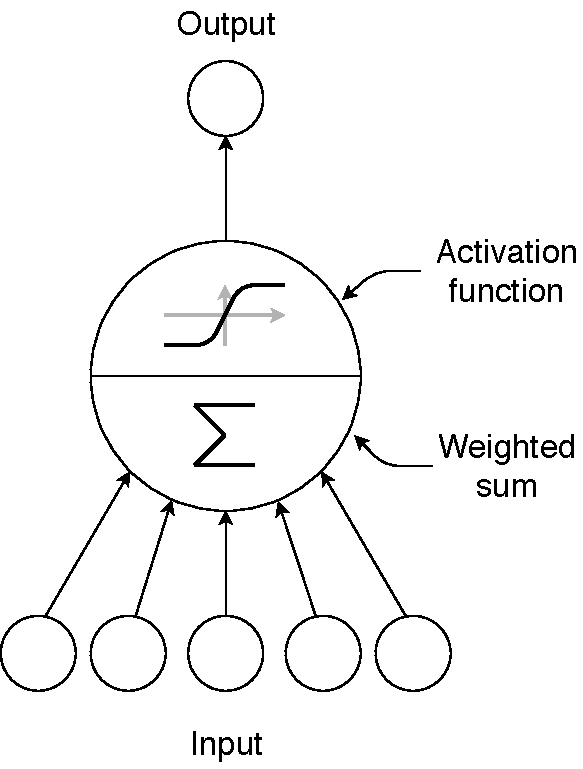
\includegraphics[scale=.6]{perceptron}
        \caption{A single neuron. Each input $x_i$ is weighted by a parameter $w_i$ before being summed and put in an activation function. The output from this funtion corresponds to the output of the neuron.}
\label{fig:neuron}
    \end{figure}

    \begin{equation}
        sigmoid(x) = \frac{1}{1 + \exp(-x)} = \frac{\exp(x)}{1 + \exp(x)}
        \label{eq:sigmoid}
    \end{equation}

    \subsection{The backpropagation method}
    The backpropagation method consists in the the propagation of the gradient of the error between the ouput of the MLP and what is expected from the output to the input of the system, hence the term backpropagation. The main equation of the gradient descent is the one presented in Equation~\ref{eq:gd_main}, with $w$ being the parameter to optimize, and $E$ the error function depending on $w$. The minus symbol represents the idea that, when using this method, one tries to achieve the lowest point of the error function, as graphically represented on Figure~\ref{fig:gd}. 

\begin{equation}
    w_{new} = w_{old} - \varepsilon \times \frac{\partial E}{\partial w}
    \label{eq:gd_main}
\end{equation}

    \begin{figure}[h]
        \centering
        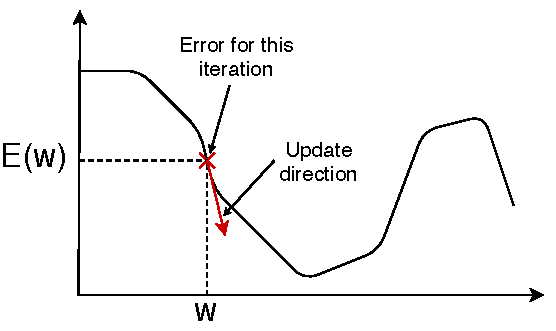
\includegraphics{gd}
        \caption{One step of gradient descent. The red cross is the current point, while the red arrow represents the direction in which the parameter has to be updated to lower the error.}
\label{fig:gd}
    \end{figure}

    The main difficulty of the update of the parameter using Equation~\ref{eq:gd_main} is to compute the value of the partial derivative of the error function $E$. This is achieved using the partial derivative composition property considering that the $E$ function can be written as follows:

    \begin{equation}
        E\left(x_{target}, x_{output}, W\right) = l\left(x_{target}, f\left(\sum_{i=1}^I w_i x_i\right)\right)
        \label{eq:error_function}
    \end{equation}

    With $l$ a loss function such as the $l_2$-norm, $f$ the activation function of the neuron, $x_i$ the $i$-th value of the input (with a total of $I$ input) and $w_i$ the corresponding weight of the neuron. For clarity of the equation, the following notation will be used:

    \begin{equation}
        a_i = \sum_{i=1}^I w_i x_i
        \label{eq:weighted_sum}
    \end{equation}

    This allows to express the partial derivative of $E$ in the following way:

    \begin{equation}
        \frac{\partial E}{\partial w_i} = \frac{\partial E}{\partial f\left( a_i\right)} \frac{\partial f(a_i)}{\partial a_i}\frac{\partial a_i}{\partial w_i} = \frac{\partial E}{\partial f\left( a_i\right)} \frac{\partial f(a_i)}{\partial a_i} x_i
        \label{eq:partial_composition}
    \end{equation}

    Equation~\ref{eq:partial_composition} being generic, it can be used with any combination of loss and activation functions. The same composition rule is also used when dealing with several layers of neurons, but in this case the partial derivate of $a_i$ by $w_i$ has to be composed again in order to ``reach'' the parameter $w_i$ in the following layer.\\

    Knowing this method, the learning of a MLP is performed by iteratively applying Equation~\ref{eq:gd_main} to all the parameters of the network until the norm of the gradient is small enough to be considered negligeable. In the following Section are presented the two kinds of Neural Networks which are trained by this method and which are used in the CRS.\@

    \subsection{MLP and Autoencoder}

    The term MLP designates the supervised Neural Network algorithm which makes possible to learn a regression between a given input and output. This definition implicitly implies that the input and the output have to be different. A special kind of Neural Networks, presented in~\cite{hinton2006reducing} and developped in~\cite{vincent2008extracting}, uses the input of the system as its output. They are called Autoencoders, because the intermediate layers of the networks, and more specifically their activations, can be used as codes to represent the input individuals. They are basically used to get a new representation of input data. They can also be used as a compression method if the encoding layer length is set to be smaller than the number of features describing the original data~\cite{hinton2006reducing}. Formally, an Autoencoder is trained by minimizing a loss function, in our case, the Mean Square Error (MSE). With our notations, the MSE for a view $V_i$ would be defined as follows:
		
		\begin{equation}
            \frac{1}{|V_i|}\sum_{x \in V_i}{(x - \hat{x})}^2
		\end{equation}
		
        With $\hat{x}$ being the output of the Autoencoder used in the $i$-th view for the input vector $x$ and $|V_i|$ being the number of elements of $V_i$.

    A graphical representation of both the MLP and the Autoencoder are presented on Figure~\ref{fig:mlp_ae}, and their uses in the Collaborative Reconstruction system are detailed in Section~\ref{sec:crs}.

    \begin{figure}[h]
        \centering
        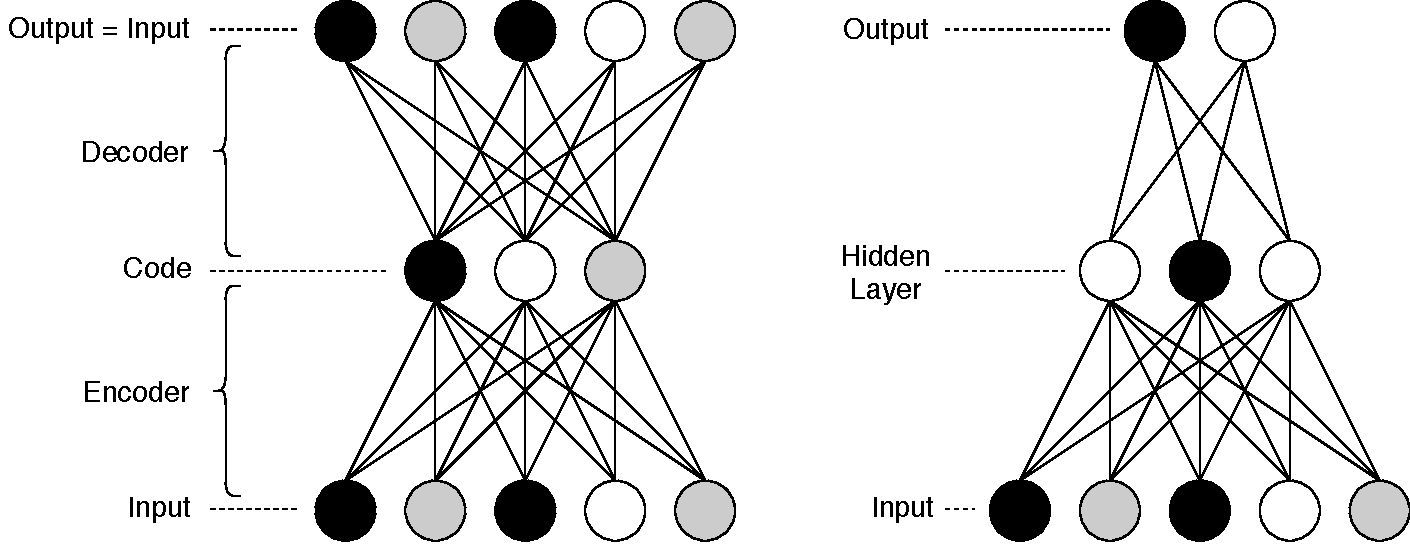
\includegraphics[scale=.5]{mlp_ae}
        \caption{An Autoencoder (left) and a Multi-Layer Perceptron (right). The intensity of the grey in each neuron symbolizes its activation.}
\label{fig:mlp_ae}
    \end{figure}
    
	\section{Cooperative Reconstruction System}
\label{sec:crs}
	
In this section, we describe the architecture of our proposed Cooperative Reconstruction System. A representation of this system can be found on Figure~\ref{fig:base}. Our system is based on several modules: first, to solve the problem of security-friendly information transfer, the system uses a set of $N$ Autoencoders~\cite{hinton2006reducing} --with $N$ being the number of views--, to locally encode data to make them impossible to read from outside of their views.
	
Then, when an individual is missing in a view, each external view sends its locally encoded version of the individual to the incomplete view, resulting in the transfer of $N-1$ encoded vectors. Then for each external view, a first approximation of the local values of the individual is inferred using a Neural Network (one per external view), in this case a Multi-Layer Perceptron. The role of this Neural Network is to make the link between the values of the external codes, and the features of the local view. After this step, the local views has access to $N-1$ versions of the missing individuals.
	
	\begin{figure}[h]
		\centering
		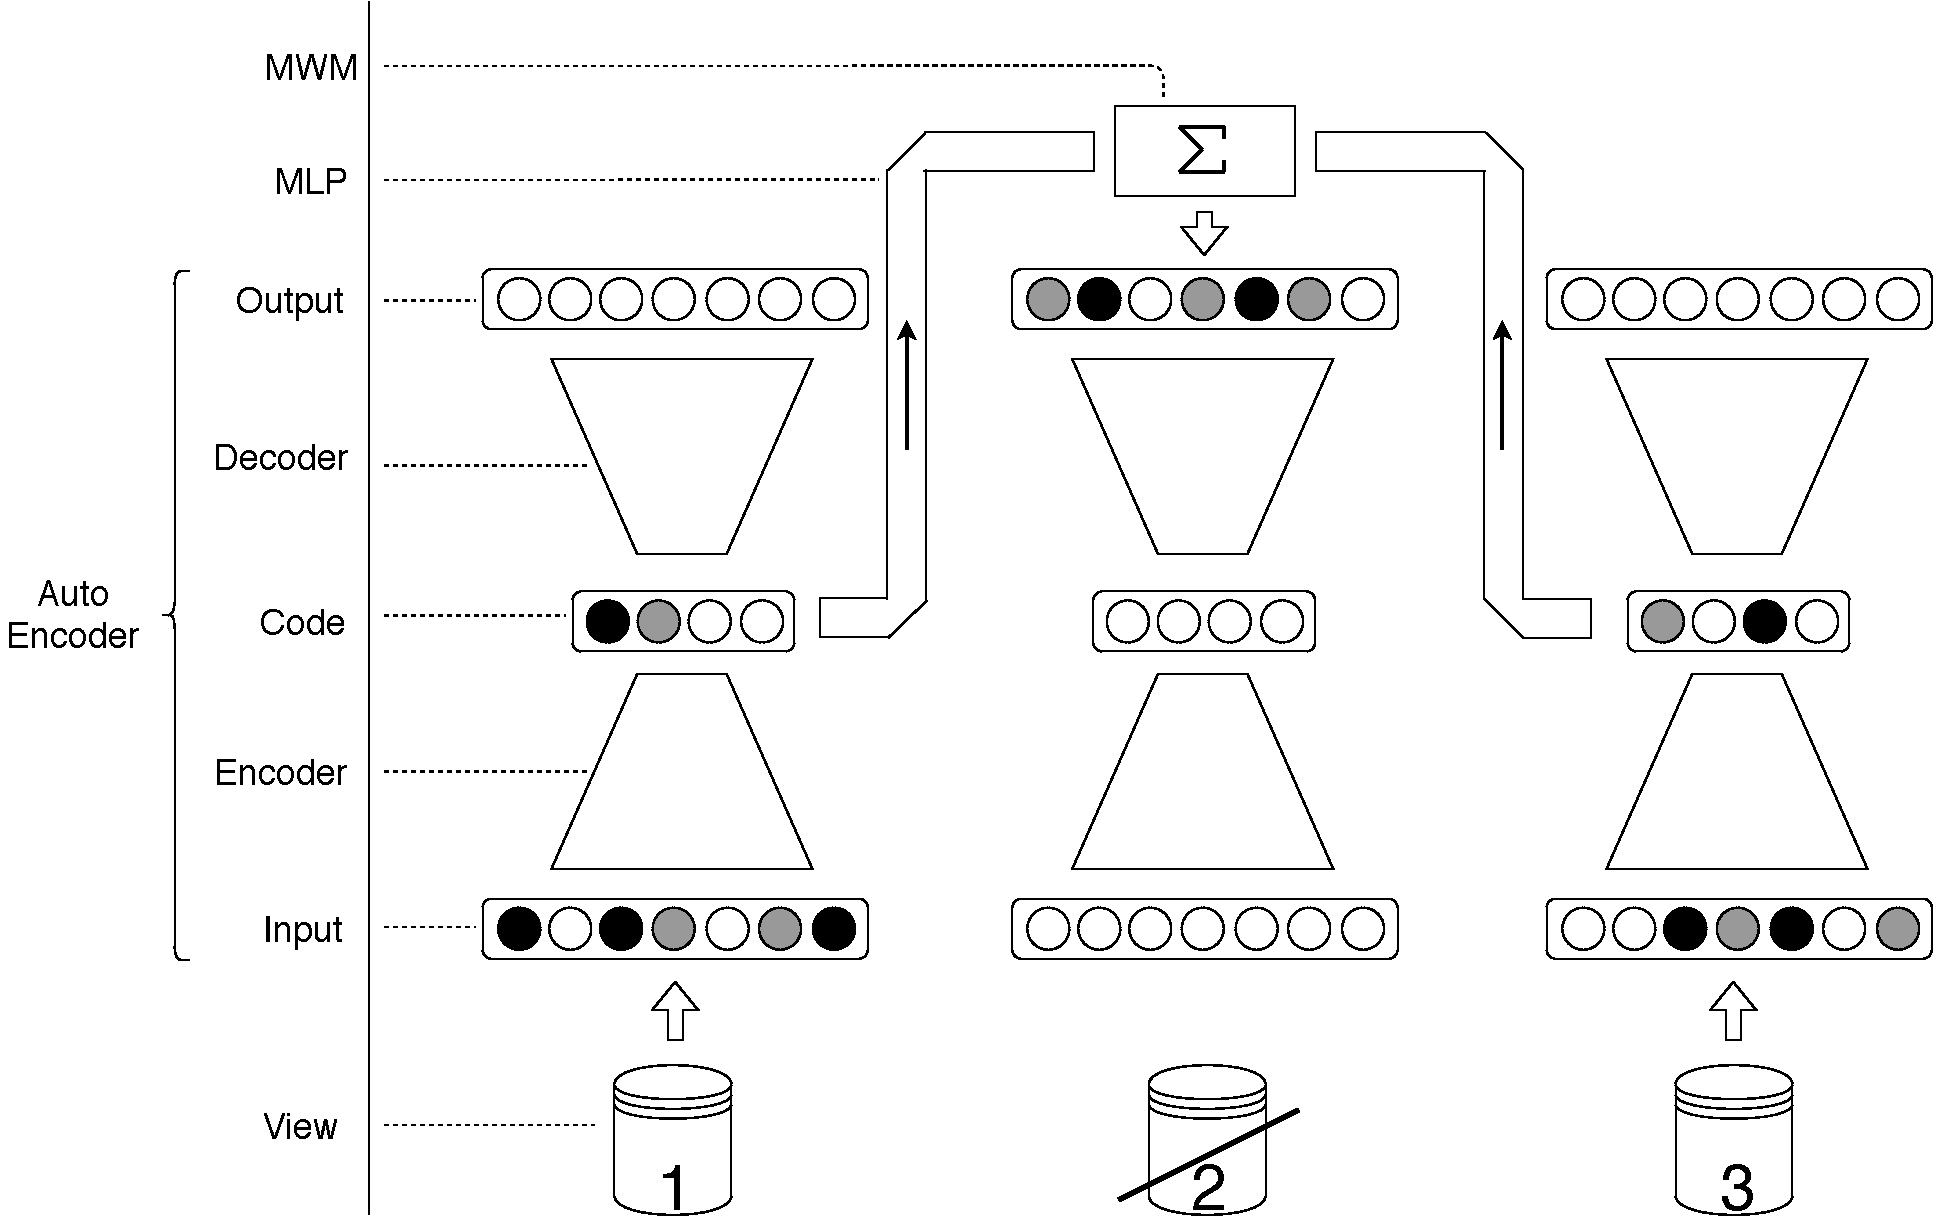
\includegraphics[width=\textwidth]{img/base_system.pdf}
        \caption{Cooperative Reconstruction System. In this example, Views 1 and
        3 are sending their coded version of the individual to View 2.}
\label{fig:base}
	\end{figure}
	
    The combination of the inferred individuals can then be used to reconstruct an accurate representation of the missing individual. However, since disagreement may occur between the different sources of information, the inferred data from each view need to be weighted to ensure an optimal reconstruction. This is solved using a weighting method we introduce in Section~\ref{sec:mwm} and called the Masked Weighting Method. The basic idea of this method is to learn a set of $N-1$ scalar vectors, called masks, to weight each approximation generated locally (cf. Fig.~\ref{fig:mwm}). These masks can be trained using either Gradient Descent or using an iterative update rule. The description of both methods can be found in Section~\ref{sec:mwm}.
	
	
The global system is designed to be modular: when a new view is available, the system just has to learn its auto-encoder and the neural networks responsible for the links between this new view and the existing ones. However, due to the nature of the weighting methods between the views, all masks have to be learned again.  This modularity is important because of the usually long learning time of a Deep Neural Network: learning the masks again does not take long, while having to re-train all neural networks would take a lot of time. It is therefore a huge gain of time that the already trained auto-encoders and links can be kept when a new view is added. This point has to be considered together with the fact that for a system made of $N$ views, approximately $N^2$ networks have to be trained.
	
Our system has been tested on two points: how good are the individuals reconstructed compared to their original versions, and what are the classification scores of these latter compared to the original ones. Thus, we tested both its efficiency at reconstruction and whether or not reconstructed data could be used for further Machine Learning.

\subsection{Notations}
\label{sec:precond}
Formally, $V_i$ and $V_j$ are the datasets of the $i$-th and $j$-th views respectively. We note $V_{i|j}$ the subset of $V_i$ (in the feature space of $V_i$) which individuals are also present in $V_j$. The size of this set is important because it will define the quantity of information available to train the inter-views Links (cf Section~\ref{sec:links})
	
		\subsection{Autoencoders}
\label{sec:dae}
		
We have selected Autoencoders to transfer information from a view to another because they offer the advantages of encoding data as scalar values, which can be used as input for further analysis, and they make it difficult to retrieve the original data without their decoding part, thus limiting possibilities of security breach. Moreover, the Autoencoders used in each view do not need to have the same architecture nor code lengths. This flexibility allows each view to use the best autoencoding architecture to describe their data.
		
When all the Autoencoders are trained, each view $j$ is able to encode the subset $V_{j|i}$ of its dataset $V_j$, before sending the result to every other view $i$ it has to collaborate with.
		
		\subsection{Links}
\label{sec:links}
A Link is a Neural Network in charge of infering the values of missing individuals based on the encoded data it received from an external view. In our case, a Link is more specifically a Multi Layer Perceptron: to reconstruct data in a local view $i$ given information from view $j$, the Link will be trained using the version of $V_{j|i}$ encoded by the $j$-th Autoencoder as its input, and $V_{i|j}$ the original data as its output. The training process of a link is summed up on Fig.~\ref{fig:link}. We remind that $V_{i|j}$ and $V_{j|i}$ are the sets of shared individuals described in $V_i$ and $V_j$ feature spaces respectively, so they necessarily represent the exact same set of individuals.

It has to be noted that the receiving view $j$ never tries to decode the encoded version of $V_{i|j}$, it only tries to infer the individuals features used in its local view. This latter point is important because it is the one that ensure the security provided by the system.

		\begin{figure}[h]
			\centering
			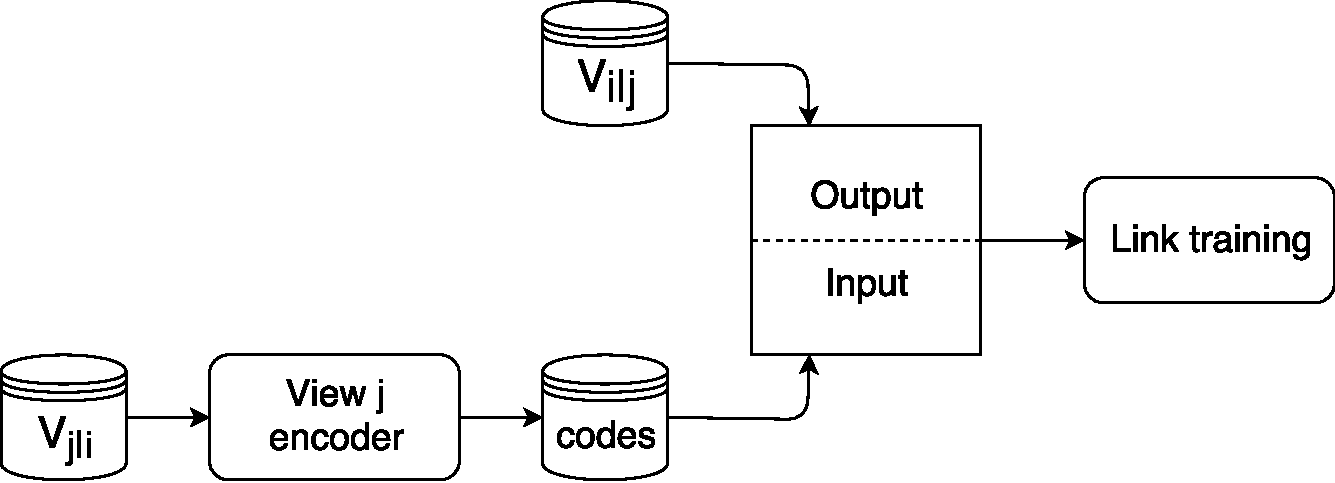
\includegraphics[scale=0.4]{img/links.pdf}
            \caption{A Link training. The dataset $V_{j|i}$ is encoded, then sent to the local view. It it used as input for the link, while $V_{i|j}$ is used as output.}
\label{fig:link}
		\end{figure}
		
        \subsection{Missing Information}
In some cases, it may happen that $V_{i|j} = \{\emptyset\}$, or is not big enough to learn the link between views $i$ and $j$. The modularity of the method presented here implies that in this case, the information coming from the external view $j$ is not taken into account, and the local view $i$ will reconstruct its missing individuals based on the information from the other external views.
		
As this case does not change the global method, for the rest of the chapter we will only consider the case in which the individuals used in the training sets are present in all views. This simplification only aims at clarifying future algebra presented in Section~\ref{sec:mwm}. When all the Links have been trained, each view has access to (at most) $N-1$ Links allowing it to infer (at most) $N-1$ version of the missing individual values.
		
		\subsection{Masked Weighting Method}
\label{sec:mwm}
When a local view $i$ has access to the $N-1$ infered versions of its missing data, it is necessary to find an efficient way to combine them to get the final version of the individual. We present a method based on a set of scalar vectors $W_i = \{w_{i|j}, \, j \in [1..N]\, \backslash \, i\}$ such that $w_{i|j}$ is of same dimension as $V_i$. To get the final output $\widetilde{x_i}$ of the system, we use the following formula:
		
    \begin{equation}
\label{eq:final}
        \widetilde{x}_i = \sum_{j \in [1..N] \backslash i} x_{i|j} \, \otimes \, w_{i|j}
    \end{equation}
	
where $\otimes$ is the pointwise vector product.
		
The coefficients can be learned using two methods: Gradient Descent on the reconstruction error, or iterative update using the zero of the derivate of this latter error. The analytical description and the characteristics of each method are described in the following section. 
		
	\begin{figure}[h]
		\centering
		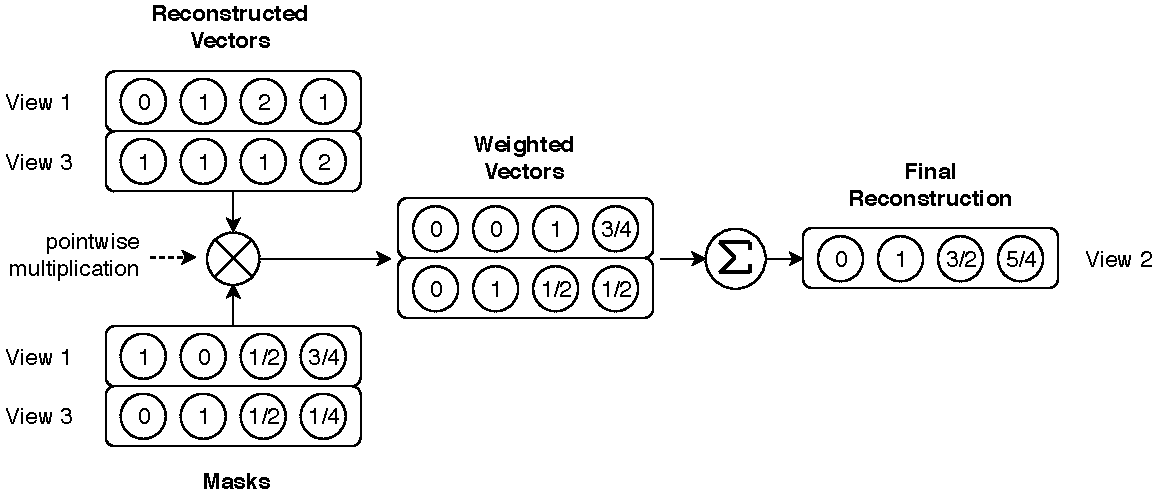
\includegraphics[width=\textwidth]{img/mwm.pdf}
        \caption{The Masked Weighting Method. View 2 has got the reconstructed
        individuals from Views 1 and 3, and it uses the masks previously trained
        to get the final weighted result.}
\label{fig:mwm}
	\end{figure}
	
        \subsubsection{Gradient Descent:}
When the reconstruction is done, it becomes possible to perform a Gradient Descent on the parameter contained in $W_i$. The error considered here is the MSE between target data and reconstructed ones. The computation of the error $E_i$ for the view $i$ can be written as follows:
		
    \begin{align*}
        E_i &= \frac{1}{|V_i|}\sum_{x_i \in V_i}||x_i - \widetilde{x}_i||^2\\
        &= \frac{1}{|V_i|}\sum_{x_i \in V_i}\sum_{k=1}^{\dim(V_i)}{(x_i^k - \widetilde{x}_i^k)}^2\\
        &= \frac{1}{|V_i|}\sum_{x_i \in V_i}\sum_{k=1}^{\dim(V_i)}{(x_i^k -
        \sum_{j \in [1..N] \backslash i} w_{i|j}^k x_{i|j}^k)}^2
    \end{align*}
		
where $x_i^k$ is the $k$-th coordinate of the individual $x_i$. The differentiation of $E$ w.r.t.\ the parameters $w_{i|j}^k$ of $W_i$ can then be written:
		
		\begin{align}
\label{eq:partialE}
            \frac{\partial E}{\partial w_{i|j}^k} &= \frac{2}{|V_i|}\sum_{x_i
            \in V_i} x_{i|j}^k \: \big(\sum_{j \in [1..N] \backslash i}
            w_{i|j}^k x_{i|j}^k - x_i^k\:\big) \nonumber \\
			&= \frac{2}{|V_i|}\sum_{x_i \in V_i} x_{i|j}^k \, \big(\,\widetilde{x}_i^k - x_i^k\:\big)
		\end{align}
		
		This latter formula makes possible to update the weight $w_{i|j}^k$ using the usual gradient formula
		
		\begin{equation}
            {(w_{i|j}^k)}^{new} = {(w_{i|j}^k)}^{old} - \epsilon \, \frac{\partial E}{\partial w_{i|j}^k}
		\end{equation}
		
		where $\epsilon > 0$ is the parameter defining the learning rate of the process. This update process is performed on every weight until convergence. In practice, the learning is stopped when the norm of the update value defined in Eq.~\ref{eq:partialE} goes under a threshold fixed by the user. 
		
		\subsubsection{Iterative update}:
It is also possible to update weights based on the minimum of $E_i$ found using
Eq.\ref{eq:partialE}.
		
		\begin{align}
\label{eq:partialE0}
            &\frac{\partial E_i}{\partial w_{i|j}^k} = 0\notag\\
            \Rightarrow\quad &\frac{2}{|V_i|}\sum_{x_i \in V_i} x_{i|j}^k \,
            \big(\,\widetilde{x}_i^k - x_i^k\:\big) = 0\notag\\
            \Rightarrow\quad &\sum_{x_i \in V_i}
            \Big({(x_{i|j}^k)}^2w_{i|j}^k+x_{i|j}^k\big(\sum_{j'\in[1..N]\backslash
            \{i,j\}} w_{i|j'}^k x_{i|j'}^k - x_i^k \big)\Big) = 0\notag\\
            \Rightarrow \quad & w_{i|j}^k \sum_{x_i \in V_i}{(x_{i|j}^k)}^2
            = \sum_{x_i \in V_i} x_{i|j}^k\big(x_i^k -
            \sum_{j'\in[1..N]\backslash \{i,j\}} w_{i|j'}^k x_{i|j'}^k
            \big)\notag\\
            \Rightarrow \quad & w_{i|j}^k = \frac{\sum_{x_i \in V_i}
            x_{i|j}^k\big(x_i^k - \sum_{j'\in[1..N]\backslash \{i,j\}}
            w_{i|j'}^k x_{i|j'}^k \big)}{\sum_{x_i \in V_i}{(x_{i|j}^k)}^2}
		\end{align}
		
Eq.\ref{eq:partialE0} shows that the update of $w_{i|j}^k$ requires the values of $\{w_{i|j'}^k, j'\in[1..N]\backslash \{i,j\}\}$. Thus it is possible to define an iterative update for which the values of $\{w_{i|j'}^{k,t}, j'\in[1..N]\backslash \{i,j\}\}$ at time $t$ are used to obtained $w_{i|j}^{k,t+1}$ at time $t+1$. This problem being convex, the iterative process is performed until convergence of the weights.\\
		
This weighting method is used because it offers several advantages:
		\begin{enumerate}
    \item In the case where an external view is too noisy, or if the Link between this external view and the local one is not good enough to infer local individuals, the weighting coefficients for this view will converge to a value under $\frac{1}{N-1}$, lowering the impact of the bad reconstruction on the result. This latter value is the default value used to weights individuals, which corresponds to the mean of the incoming values to aggregate.
    \item On the opposite, if a small subgroup of views is highly linked to the local one, this weighting method will favor these views to maximize the quality of the reconstructed individuals~\cite{sublime2017analysis,sublime2018analysis}.
    \item Contrary to a weighted mean which would assign a single scalar to each view, this method allows to favor only a subpart of the reconstructed vector. Indeed, one can easily imagine that sometimes, the information contained in a view would only allow to recover part of the information contained in the local view, which entails a better reconstruction score on specific features of the local individual. Our weighting method makes possible to automatically identify these parts during parameters training.
		\end{enumerate}
		
When $W_i$ has been trained for all the views, the system is ready to be used on missing data. An abstraction of the reconstruction process can be found on Figure~\ref{fig:process}, and a summary of the system architecture can be found on Figure~\ref{fig:base}. This latter can be used to see that there is no original data crossing the line between the local view and the external ones.
	
	\begin{figure}[h]
		\centering
		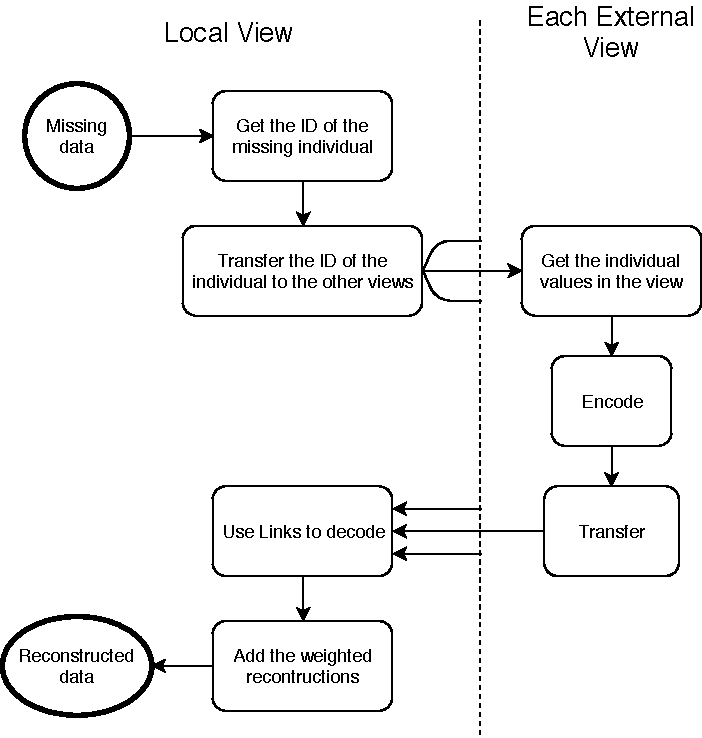
\includegraphics[scale=0.8]{img/process.pdf}
        \caption{Reconstruction process going from the identification of a
        missing data to the getting of its reconstructed version.}
\label{fig:process}
	\end{figure}	
	
	\section{Experimental setting}
\label{sec:exp}
This Section presents the experiments that have been conducted to test our proposed method.\@ First are presented in Section~\ref{sec:datasets} the datasets which have been used during the experiments, then the global methodology used to analyze the system behavior is described in Section~\ref{sec:methodo}. The measures used to quantify the results are presented in Section~\ref{sec:measures}, and finally numeric results are presented in Section~\ref{sec:results}.

	\subsection{Datasets}
\label{sec:datasets}
To get empirical results of the Collaborative Reconstruction System, we use it on three different datasets usable in a multi-view context, namely Wisconsin Diagnostic Breast Cancer (WDBC), Multi-Features Digital Dataset (MFDD), Madelon and Cube. While the description of the first three datasets can be found in Appendix~\ref{sec:app-datasets}, Cube is presented here because it is related to this chapter only.
	\begin{enumerate}
        \item \textit{Wisconsin Diagnostic Breast Cancer (WDBC)}: This dataset has 569 instances with 32  variables (ID, diagnosis, 30 real-valued input variables). Each data observation is labeled as benign (357) or malignant (212). Variables are computed from a digitized image of a fine needle aspirate (FNA) of a breast mass.  They describe characteristics of the cell nuclei present in the image. Since each data contains the characteristics of 3 nuclei, we have 3 natural views here.
        \item \textit{Multi-Features Digital Dataset (MFDD)}: This dataset consists of features of handwritten numerals (from 0 to 9) extracted from a collection of Dutch utility maps. 200 patterns per class (for a total of 2,000 patterns) have been digitized in binary images. These digits are represented in terms of the following six feature sets, each set being here used as a view: 76 Fourier coefficients of the character shapes, 216 profile correlations, 64 Karhunen-Love coefficients, 240 pixel averages in 2 $\times$ 3 windows and 47 Zernike moments morphological features. Each set of coefficient stands for a view.
        \item \textit{Madelon}: This dataset is an artificial dataset containing data points grouped in 32 clusters placed on the vertices of a five dimensional hypercube and randomly labeled +1 or -1. The five dimensions constitute 5 informative features. 15 linear combinations of those features were added to form a set of 20 (redundant) informative features. Based on those 20 features one must separate the examples into the two classes (corresponding to the +-1 labels). Finally 480 features called `probes' having no predictive power were added by the authors. The order of the features and patterns is random. This dataset is the most challenging among these used here. It is used to test the ability of our sytem to ignore noise (it should not reconstruct it) and to show that despite the large number of noisy features, we still have good classification results regardless of the poor reconstruction. Because no further information in available on this dataset, the views are randomly generated by picking a random set of 125 features for each.
        \item \textit{Cube}: In addition of the three previously described datasets, we have created a toy example which we mainly use to test the effectiveness of the Masked Weighting Method. This dataset, which we will refer to as the Cube dataset, is made of 1000 3-dimensional points divided in 4 classes of 250 members each. The points of each class are generated using a normal law with a standard deviation of $0.1$ and centered either on the center of the feature space $(0,0,0)$, or at the extremity of one on the three unit vectors $(1,0,0)$, $(0,1,0)$ and $(0,0,1)$. A graphical representation of the Cube dataset can be seen on Figure~\ref{fig:cube}. The 3 views are obtained by projecting the whole dataset according to one of the three previous unit vectors. The point of this segmentation is explained in Section~\ref{sec:results}.
	\end{enumerate}

    \begin{figure}[h]
        \centering
        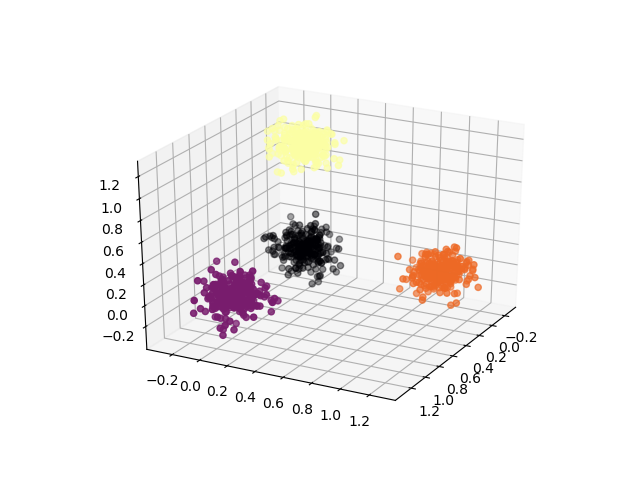
\includegraphics[scale=.7]{img/data}
        \caption{The Cube dataset}
\label{fig:cube}
    \end{figure}
	
	\subsection{Methodology}
\label{sec:methodo}
In order to analyze each aspect of the system, several sets of experiments have been conducted.	The first set consists in training a system with and without the Masked Weighting Method and to analyze the results in terms of reconstruction quality (Section~\ref{sec:msemrd}). When it comes to combining the results from each external views, the system without our combination method simply uses a normalized equi-weighted sum of the reconstructed external vectors. This first experiment has been conducted in order to both test the viability of the method and determine the impact of our new combination method.\@ An intermediary result is presented in Section~\ref{sec:num}: the reconstruction of images from the MFDD dataset is graphically presented. The second set of experiments consists in the analysis of the results obtained during the first set, but this time considering the impact of the Masked Weightinh Method on a classification task performed on the reconstructed data (Section~\ref{sec:classif}). Finally, the third and last set of experiments consists in the analysis of the masks values for the toy example (Section~\ref{sec:results_mwm}). This is done to ensure the method is able to determine which reconstructor is better for which part of the reconstructed individuals.
	
For all sets of experiments, the global methodology remains the same: each view is split in a training set (90\%) and a test set (10\%), then all neural networks (Autoencoders and Links) are trained using the required training set. To test the system, the process described in Figure~\ref{fig:process} has been conducted on the test dataset of each view, with the results being compared to the original data.
	
As there might be some variabilities in the results depending on the initialization of each neural network, the experiments have been conducted several times and the results have been averaged. Experiments on the WDBC dataset were repeated 50 times, while these performed on MFDD 20 times, these on Madelon 10 times and these on Cube 50 times. This difference is due to different dataset sizes, which increases the training time necessary for each neural network.
	
	\subsection{Measures}
\label{sec:measures}
To determine the performance of our system, we used three measures. The first one is the Mean Squared Error (MSE) between the reconstructed vector and its target. Given two $K$-dimensional vectors $x$ and $y$ with respective coordinates sets ${\{x_i\}}_{i \in [1..K]}$ and ${\{y_i\}}_{i \in [1..K]}$, their MSE can be computed as follow:
	
	\begin{equation}
        MSE(x, y) = \frac{1}{K}\sum_{i = 1}^{K}{(x_i - y_i)}^2
	\end{equation}

The global error is then the average of the MSE of all the reconstructed vectors compared with their target values. The point of this measure is to get a global idea of the distance between the reconstructed vectors and the target ones.
	
The second error we use is the Mean Relative Difference (MRD) between the feature values of the reconstructed vector and these of the target vector. Given the same $x$ and $y$ than above, their MRD is computed as follow: 

	\begin{equation}
		MRD(X, Y) = \frac{1}{K}\sum_{i=1}^{K}\Big|\frac{x_i - y_i}{y_i}\Big|
	\end{equation}
	
Here again, the global error is the average of the MRD of all the reconstructed vectors compared to their target values. This measure is used pairwise with the MSE in order to get more precise information about the difference between the reconstructed vector and the target one. Because of the security constraint and because of the difficulties the system may have to link the views, we do not expect these errors to be as good as these obtained by reconstruction and inference systems with less constraints such as standard Multi-Layer Peceptron~\cite{vincent2010stacked}.
	
To test the usability of the reconstructed vectors, they have been tested in a classification task: Random Forest classifiers were trained on the original data (one for each view), then we tested whether or not the data reconstructed using our proposed method were classified correctly by these trained Random Forest classifiers. The results were compared with performances on a test set with complete non reconstructed data.
	
The error considered here is the mean difference between the classification scores obtained in each view on their test datasets with the original data and the ones obtained with the reconstructed individuals. For the remainder of the thesis, we will name this error the Classification Difference. Contrary to the two previous ones, this error is not intended to determine the difference between a vector and its reconstruction, but rather to look at the impact of the reconstruction process on later data processing (such as a classification task). Even with mitigated reconstruction scores (MSE and MRD), a low Classification Difference would mean that the reconstructed individuals can be used in further applications. This score is presented along with the classification scores of each view. The Random Forest classifiers have been trained using the entropy cost function, with 50 estimators and with a max depth of 5.\\

Finally, to ensure the efficiency of the Masked Weighting Method when it comes to favor subparts of reconstructed vectors depending on the source external view, we simply have analyzed the vectors values of these masks for the Cube dataset. This dataset is particular because the projection performed to obtain a view entails the overlap of 2 clusters around the point $(0,0)$. Moreover, projecting according to a specific axe, which is equivalent to supress a column in the original 3-dimensional dataset, prevents the local view to have any information on this axe, while its pairs will need this information to reconstruct their local individuals. If the Masked Weighting Method works as intended, a huge difference between the values of the mask should be observed. This process is illustrated in Figure~\ref{fig:process_mwm}.

\begin{figure}[h]
    \centering
    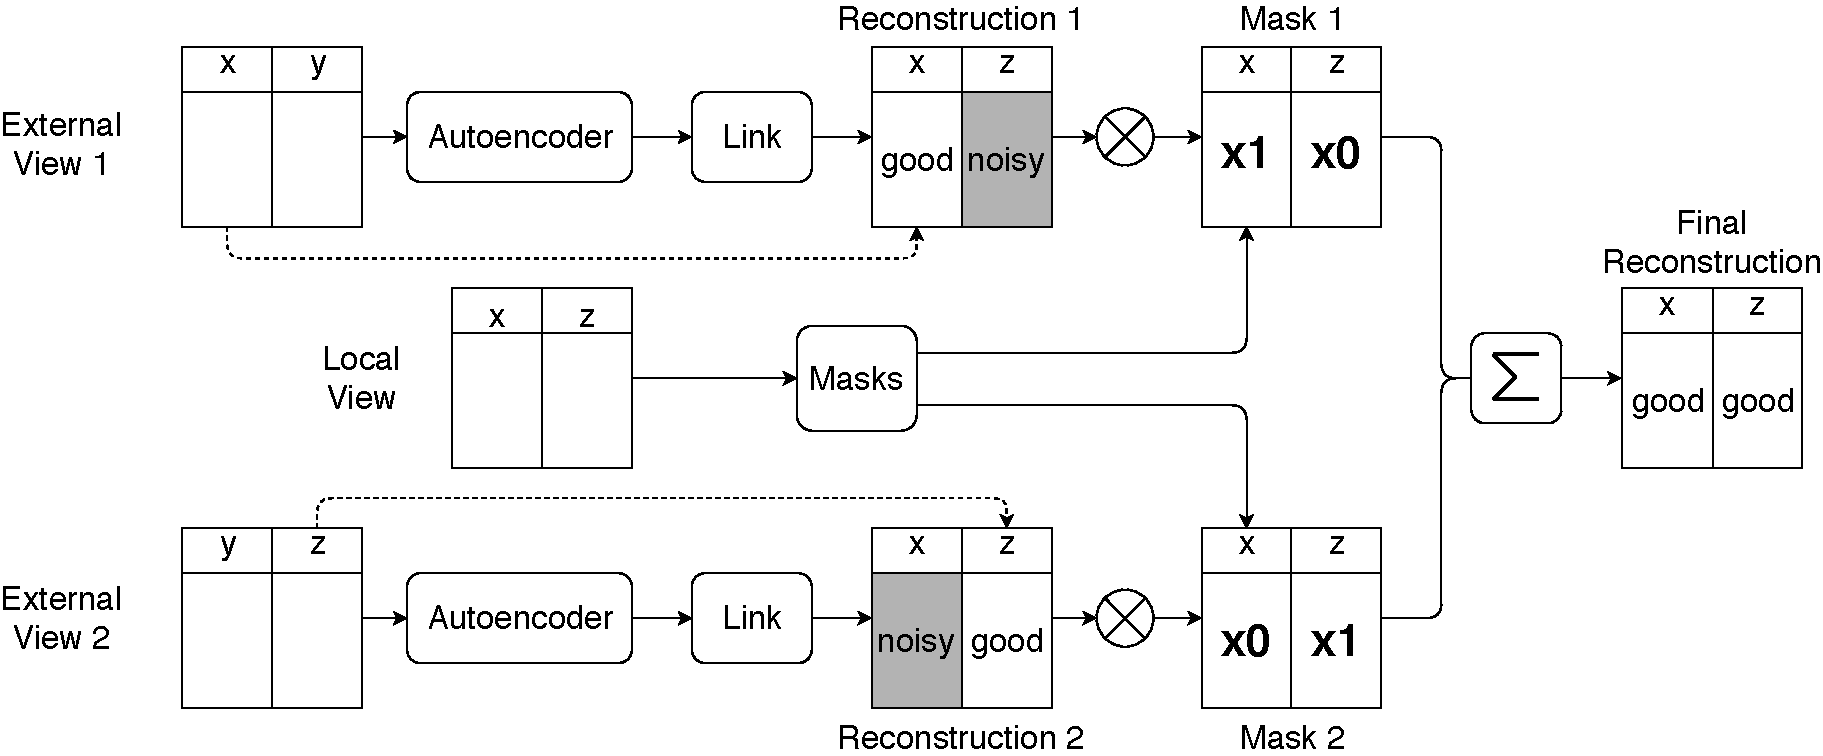
\includegraphics[scale=.38]{img/process_mwm}
    \caption{The combination of two partially good reconstructions into a good one. In this example, each view has enough information to reconstruct only one feature out of the two in the local view (doted lines). The Masked Weighted Method is designed to favor the best reconstructed part of each partial reconstruction, hence the $\times 0$ and $\times 1$ in the masks.}
\label{fig:process_mwm}
\end{figure}
	
	\section{Results}
\label{sec:results}
This Section is divided following the different kind of experiments that have been conducted. In Section~\ref{sec:msemrd} are presented the numeric results of the reconstruction process, then in Section~\ref{sec:num} are presented some visual results presented the quality of the reconstructed individuals using the MFDD database. Section~\ref{sec:classif} presents the results obtained on the classification process performed on the reconstructed individuals, and finally Section~\ref{sec:results_mwm} presents the analyzis conducted on the evolution of the masks coefficients depending on the information shared by views.

    \subsection{Basic reconstruction with and without the Masked Weighting Method}
\label{sec:msemrd}
	
During this experiment, we were interested in the impact of our combination method on the results of the system.\@ A summary of the results on WDBC, MFDD, Madelon and Cube can be found in Appendix~\ref{fig:msemrd} and~\ref{fig:classif}.

\begin{figure}[h]
\label{fig:msemrd}
    \centering
    \subfloat[][WDBC]{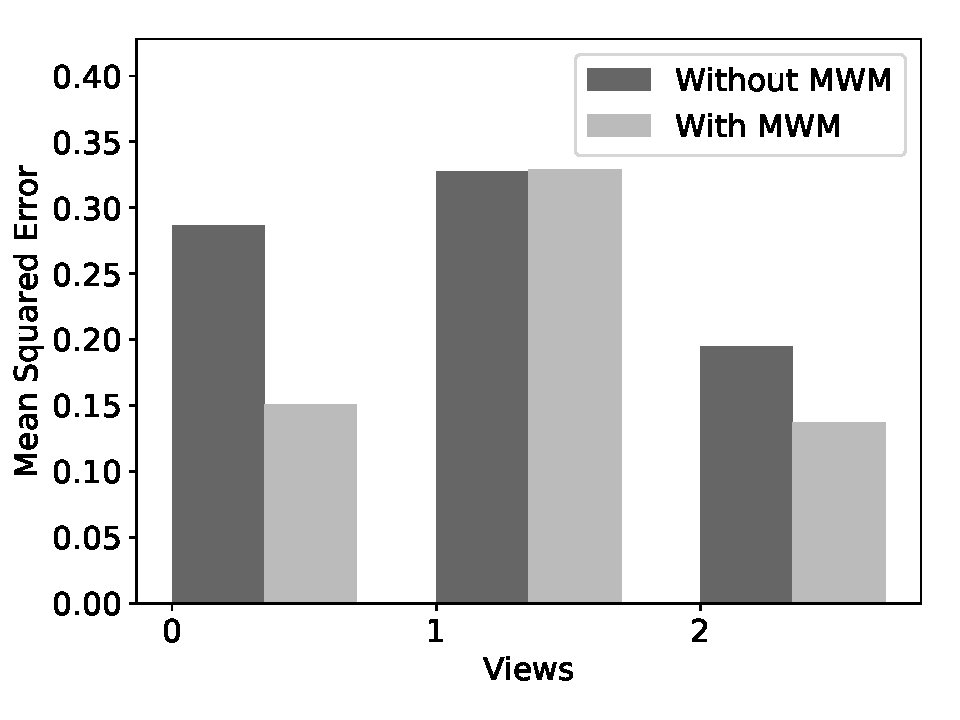
\includegraphics[scale=.30]{img/mse_wdbc}\label{fig:mse_a}}
    \qquad
    \subfloat[][WDBC]{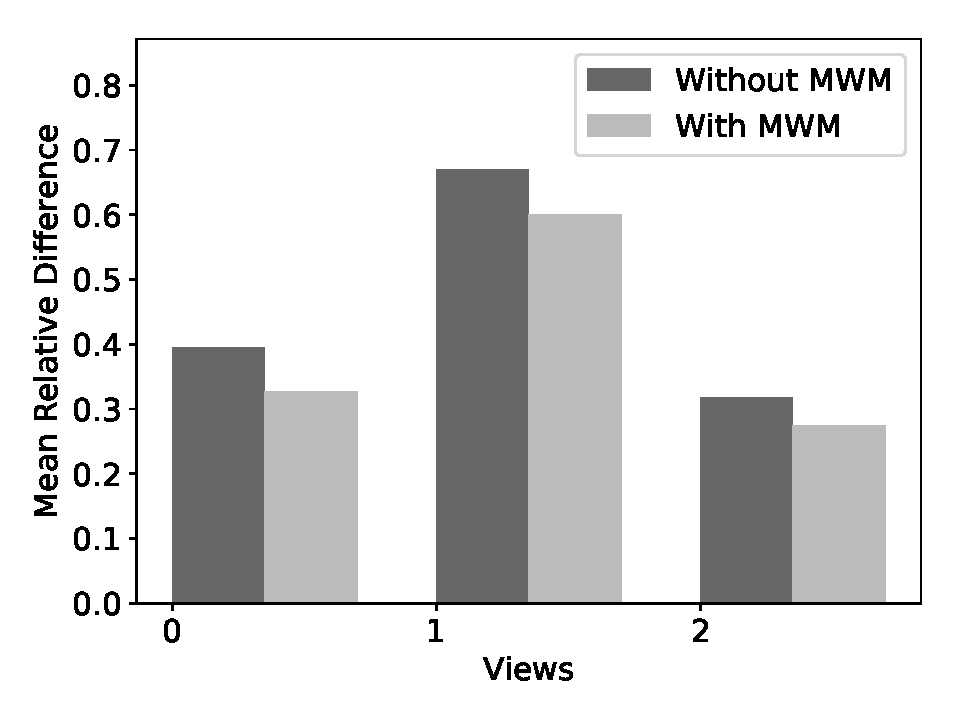
\includegraphics[scale=.30]{img/mrd_wdbc}\label{fig:mrd_a}}\\
    \subfloat[][MFDD]{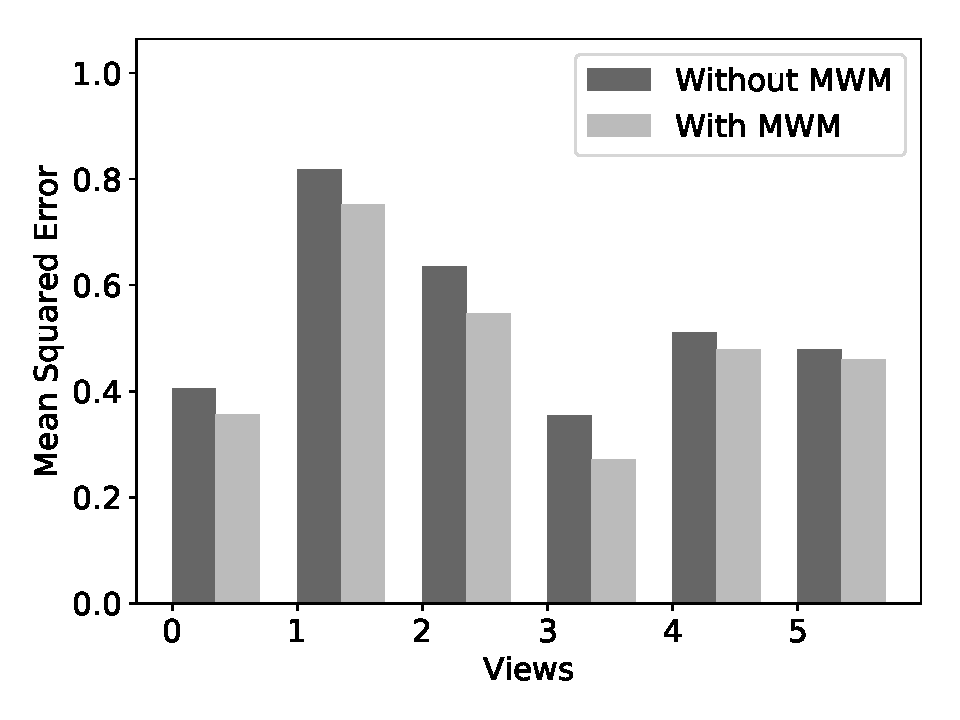
\includegraphics[scale=.30]{img/mse_mfeat}\label{fig:mse_b}}
    \qquad
    \subfloat[][MFDD]{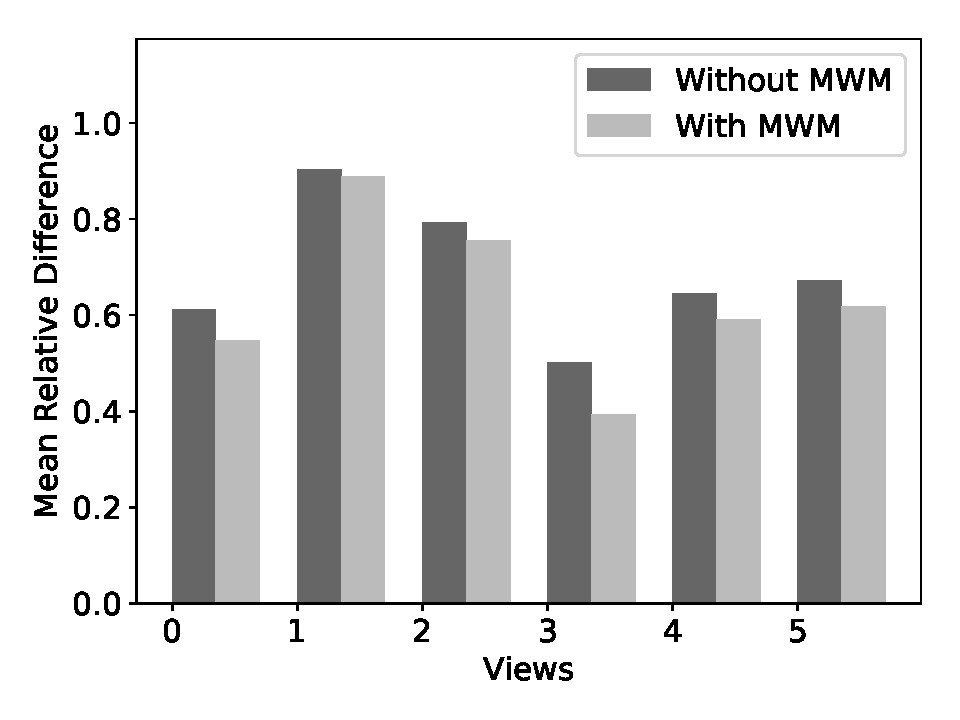
\includegraphics[scale=.30]{img/mrd_mfeat}\label{fig:mrd_b}}\\
    \subfloat[][Madelon]{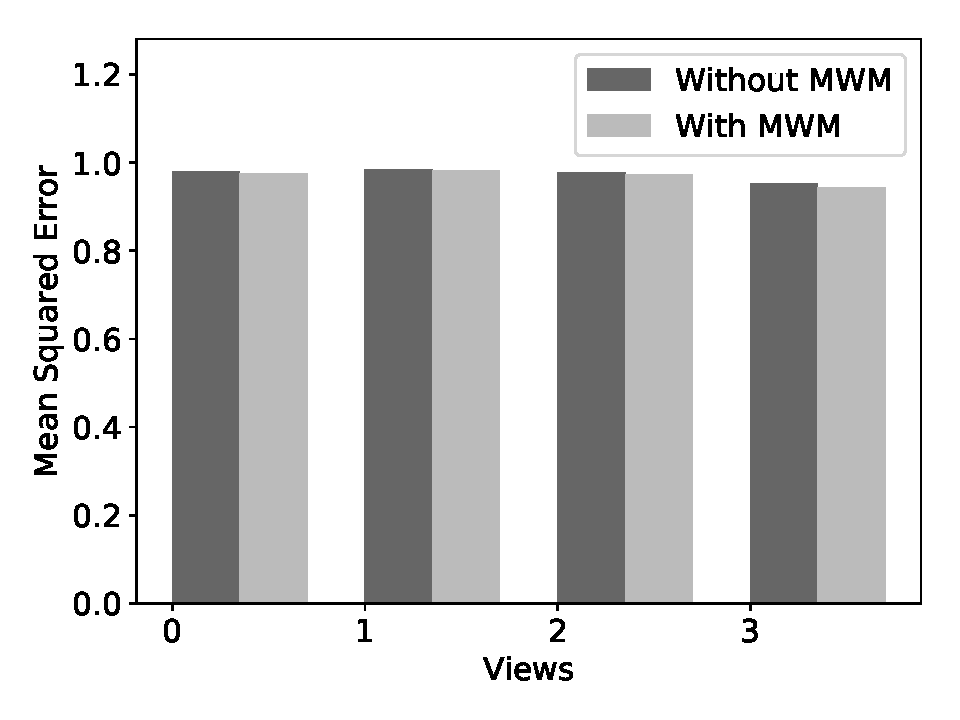
\includegraphics[scale=.30]{img/mse_madelon}\label{fig:mse_c}}
    \qquad
    \subfloat[][Madelon]{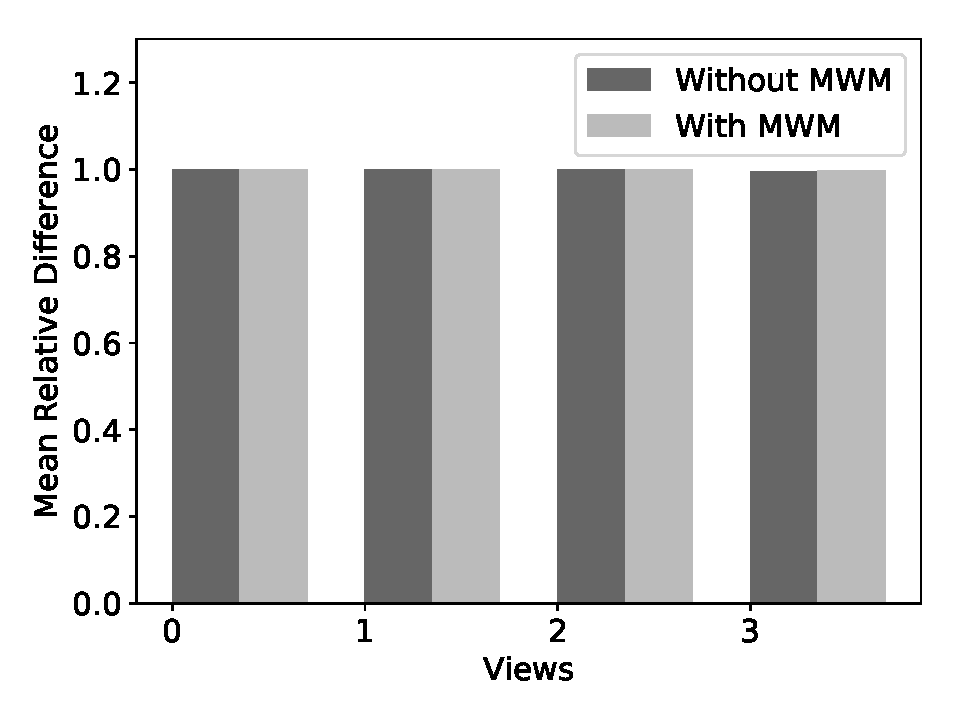
\includegraphics[scale=.30]{img/mrd_madelon}\label{fig:mrd_c}}\\
    \subfloat[][Cube]{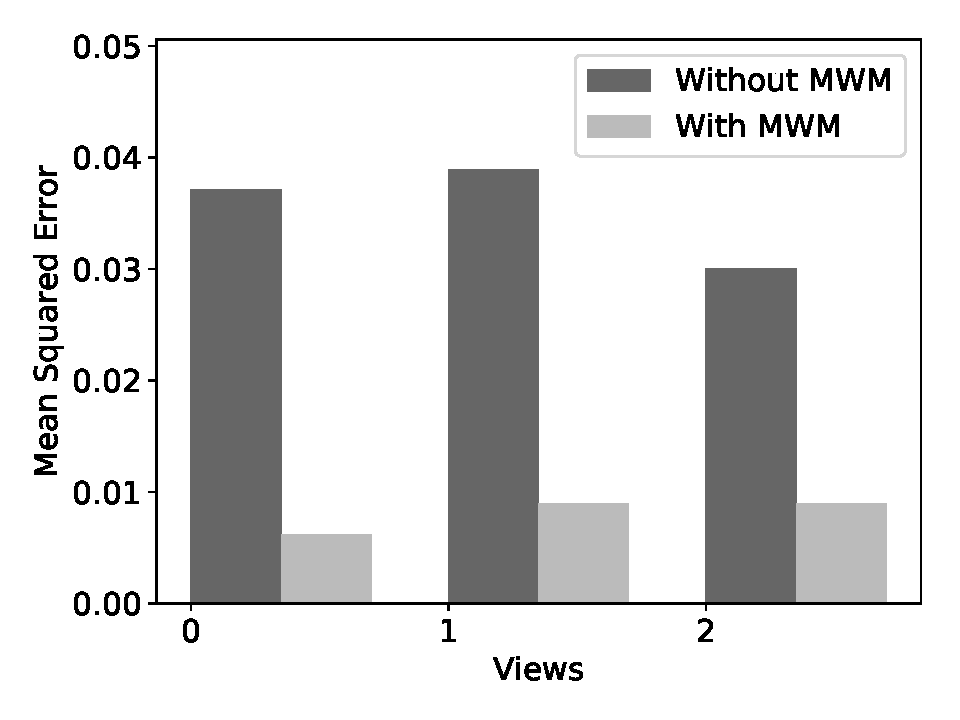
\includegraphics[scale=.30]{img/mse_cube}\label{fig:mse_d}}
    \qquad
    \subfloat[][Cube]{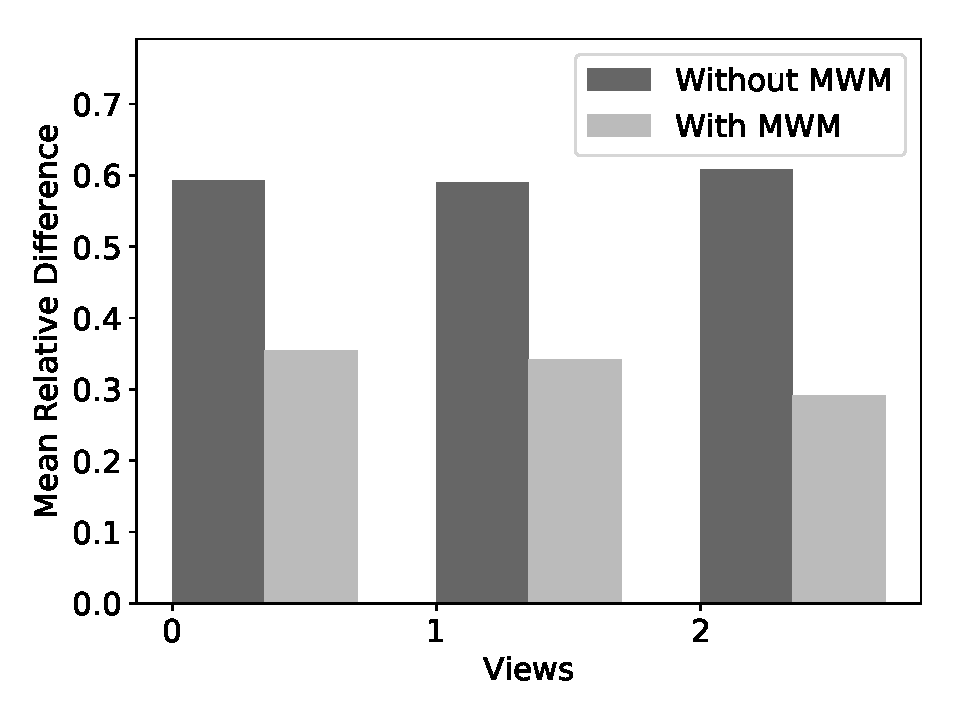
\includegraphics[scale=.30]{img/mrd_cube}\label{fig:mrd_d}}
    \caption{Mean Squared Error and Mean Relative Difference for all the datasets.\@ A lower value corresponds to a better result.}
\end{figure}

	
\begin{figure}[H]
\label{fig:classif}
    \centering
    \subfloat[][WDBC]{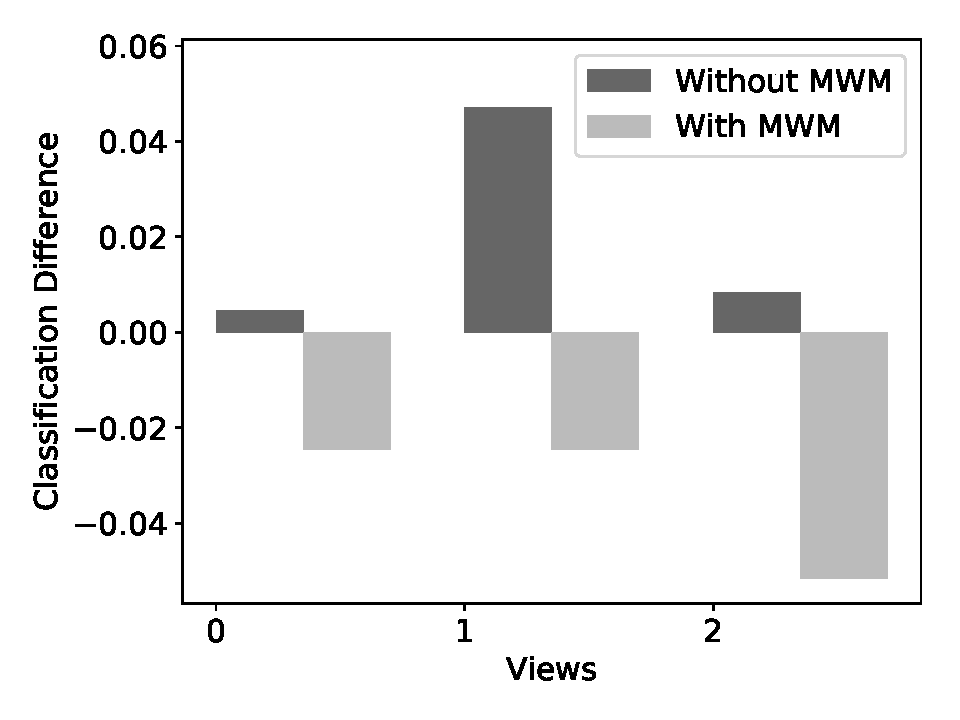
\includegraphics[scale=.30]{img/cd_wdbc}\label{fig:classif_c}}
    \quad
    \subfloat[][MFDD]{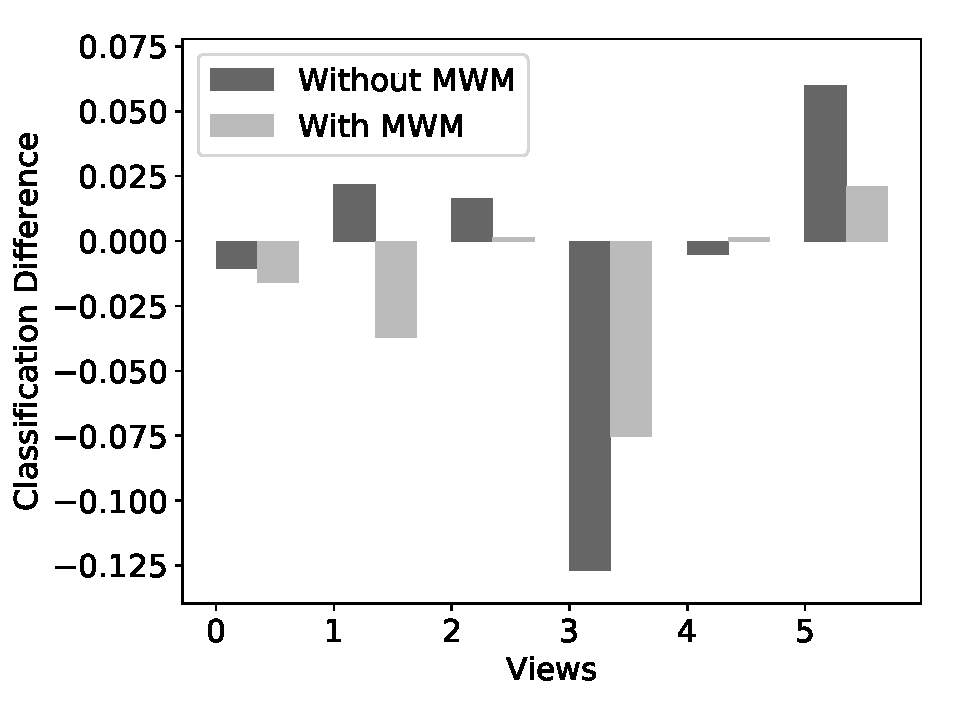
\includegraphics[scale=.30]{img/cd_mfeat}\label{fig:classif_d}}\\
    \subfloat[][Madelon]{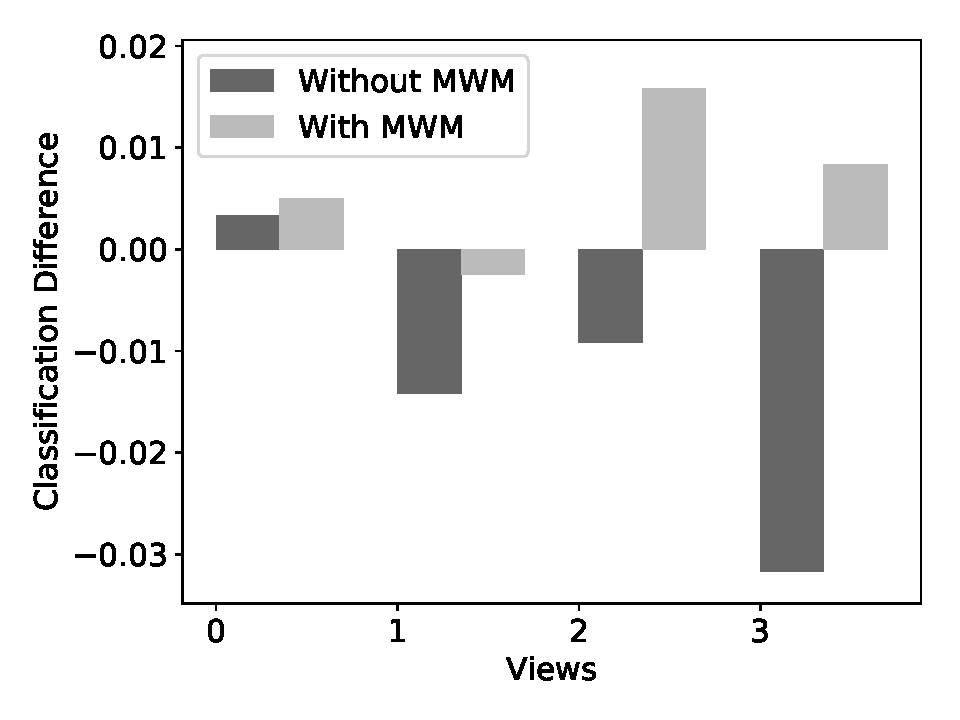
\includegraphics[scale=.30]{img/cd_madelon}\label{fig:classif_f}}
    \quad
    \subfloat[][Cube]{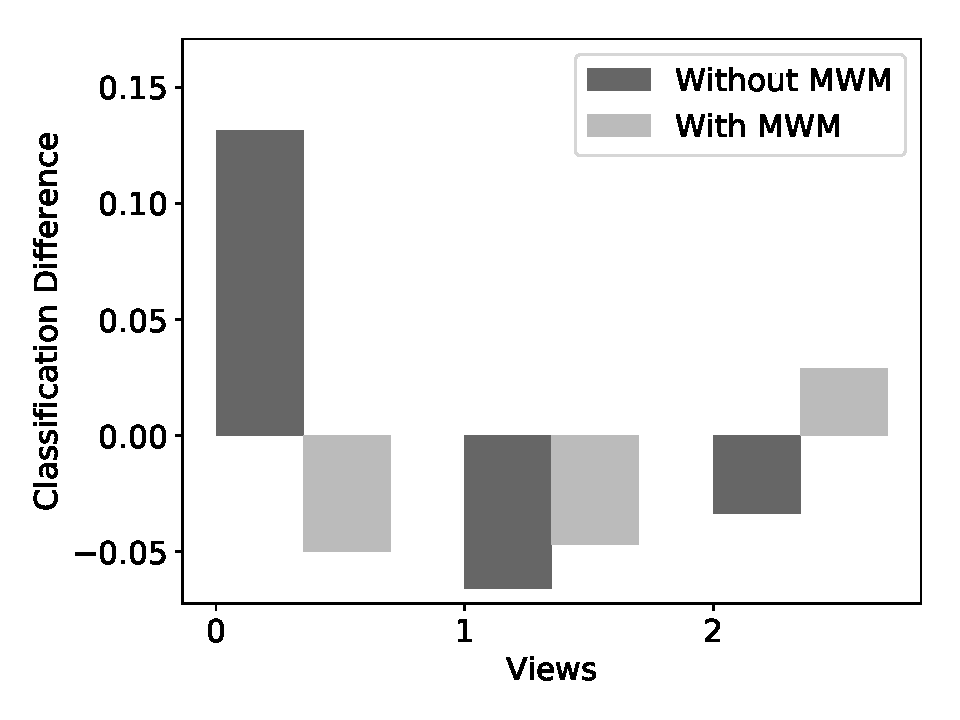
\includegraphics[scale=.30]{img/cd_cube}\label{fig:classif_h}}
    \caption{Classification Scores and Difference for WDBC, MFDD and
        Madelon: original scores from the original data, classification score from the reconstructed data without and with the Masked Weighting Method and their difference.}
\end{figure}

For WDBC, MFDD and Cube, the Masked Weighting Method significantly reduces the MSE for almost every view (Figures~\ref{fig:mse_a},~\ref{fig:mse_b} and~\ref{fig:mse_d}). This was expected because the use of this method implies the optimization of parameters w.r.t.\ this error. Moreover, the MRD is reduced for all the views in WDBC, MFDD and Cube (Figures~\ref{fig:mrd_a},~\ref{fig:mrd_b} and~\ref{fig:mrd_d}): the reconstructed individuals are closest to their original versions. The exceptionnal results obtained for the MSE on the Cube dataset (Figure~\ref{fig:mse_d}) can be explained by the fact that this dataset has been created as a perfect example for our weighting method.\@ Further results can be found in Section~\ref{sec:results_mwm}.

Considering the reconstruction results on the Madelon dataset (Figure~\ref{fig:mse_c} and Figure~\ref{fig:mrd_c}), the high MSE and MRD values were expected because of the numerous noisy features present in every view (480 out of 500): the Links could not reconstruct noise based on some more noise. The values around 1 for the MSE and MRD (Figure~\ref{fig:mse_c} and~\ref{fig:mrd_c}) can be explained by the fact that during the training, the trained Links were only returning values around $10^{-2}$ (the noise could not be reconstructed as expected), while the scaled dataset mostly consists of values around 1. This case presents an extreme situation for which our system does not work as intended: the fact that it tries to reconstruct every feature of the local view implicitly implies that these features are not too noisy and can also be explained using the information available in the external views, which is not the case for the Madelon dataset.
	
\subsection{Graphical Reconstruction of Handwritten Digits}
\label{sec:num}

To better analyze the quality of the reconstructed individuals, we have used a specific view of the MFDD dataset, namely the one with the 240 pixel averages in 2 $\times$ 3 windows. The individuals of the tests datasets have been reconstructed and plotted. A sample of the individuals in the original dataset is presented on Figure~\ref{fig:num_original}. The contrast difference is explained by the normalization of the descriptive vectors before plotting.

\begin{figure}[H]
    \centering
    \subfloat[][]{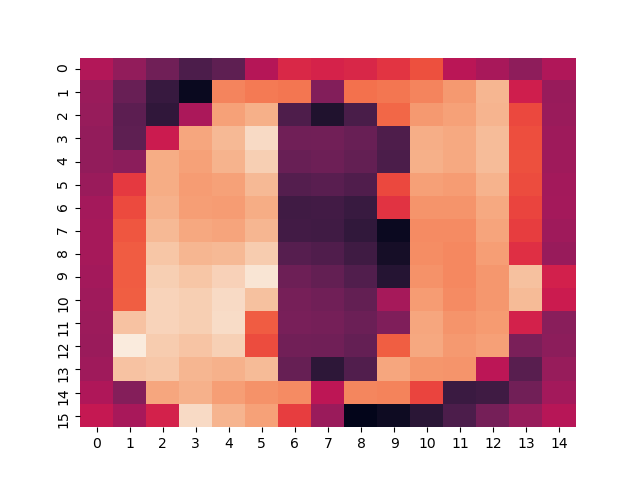
\includegraphics[scale=.15]{img/sample_original/o0}}
    \subfloat[][]{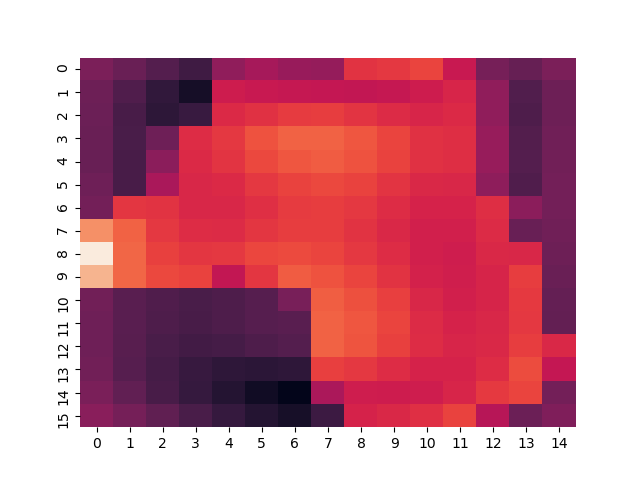
\includegraphics[scale=.15]{img/sample_original/o1}}
    \subfloat[][]{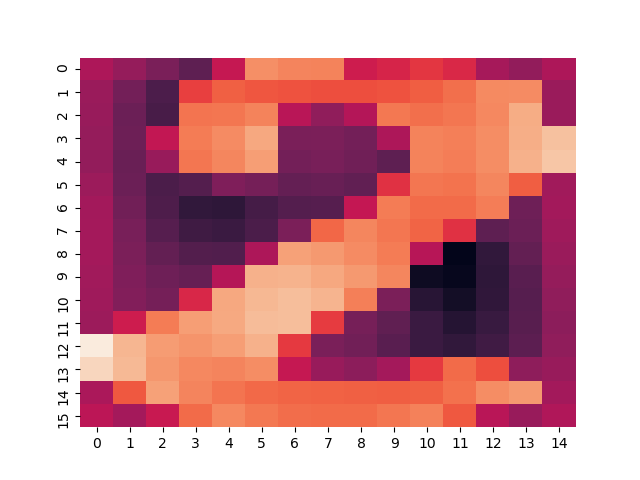
\includegraphics[scale=.15]{img/sample_original/o2}}
    \subfloat[][]{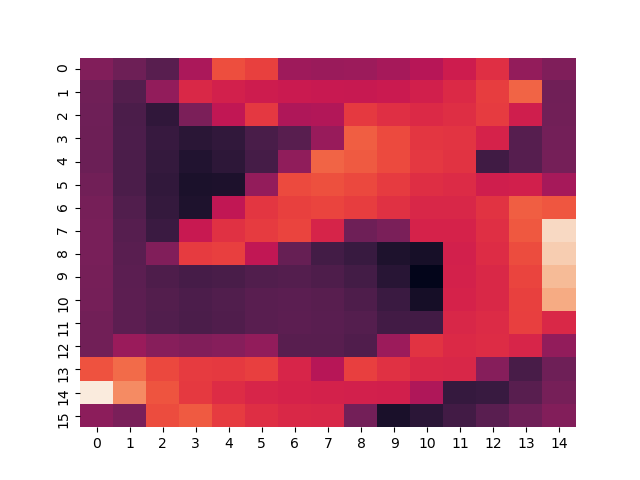
\includegraphics[scale=.15]{img/sample_original/o3}}
    \subfloat[][]{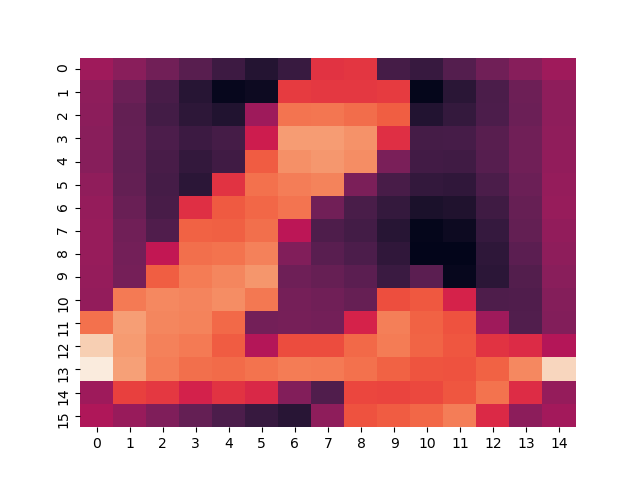
\includegraphics[scale=.15]{img/sample_original/o4}}\\
    \subfloat[][]{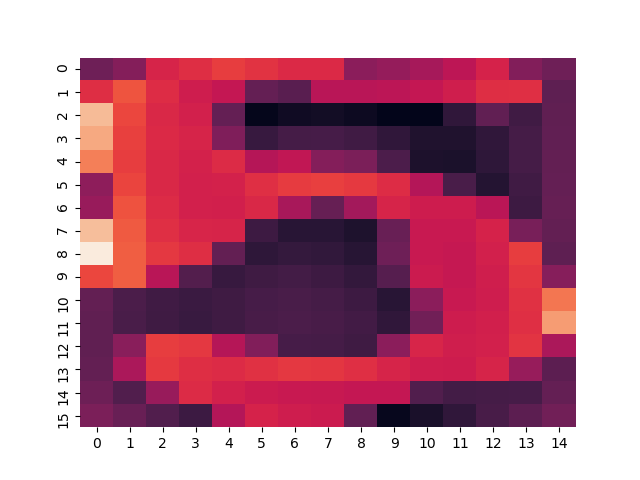
\includegraphics[scale=.15]{img/sample_original/o5}}
    \subfloat[][]{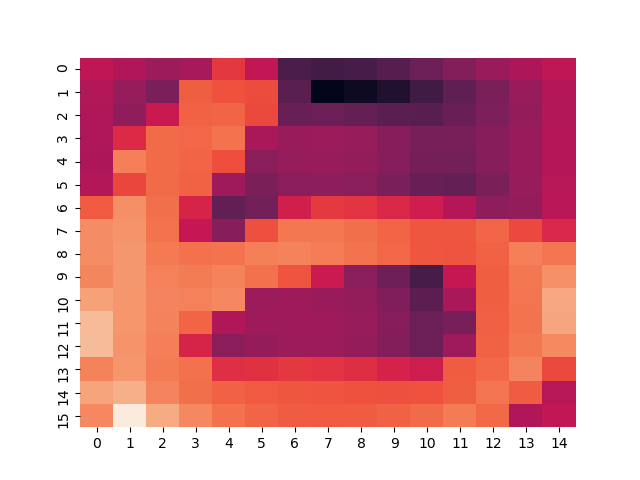
\includegraphics[scale=.15]{img/sample_original/o6}}
    \subfloat[][]{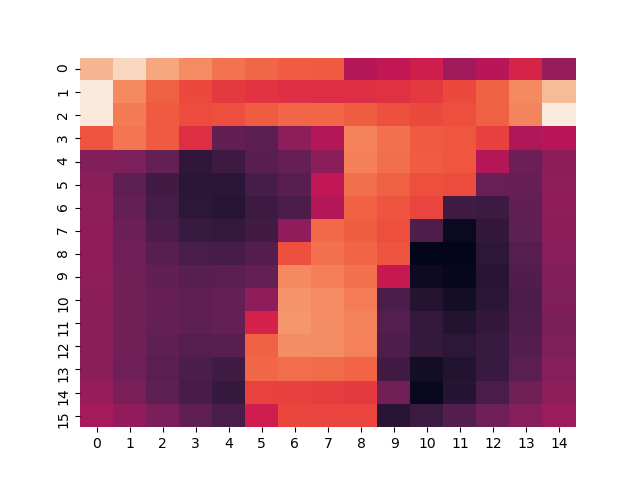
\includegraphics[scale=.15]{img/sample_original/o7}}
    \subfloat[][]{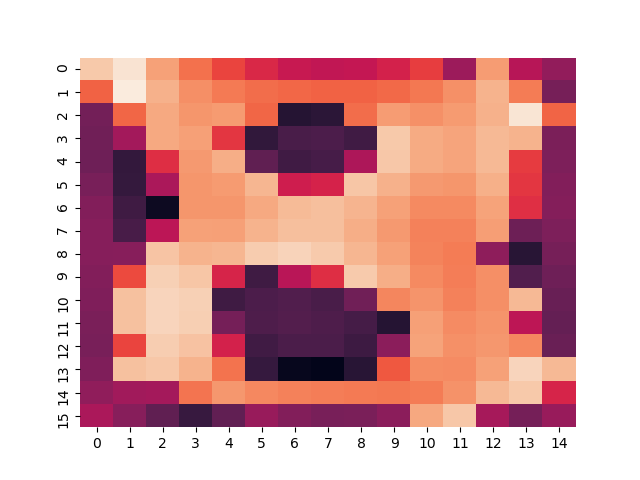
\includegraphics[scale=.15]{img/sample_original/o8}}
    \subfloat[][]{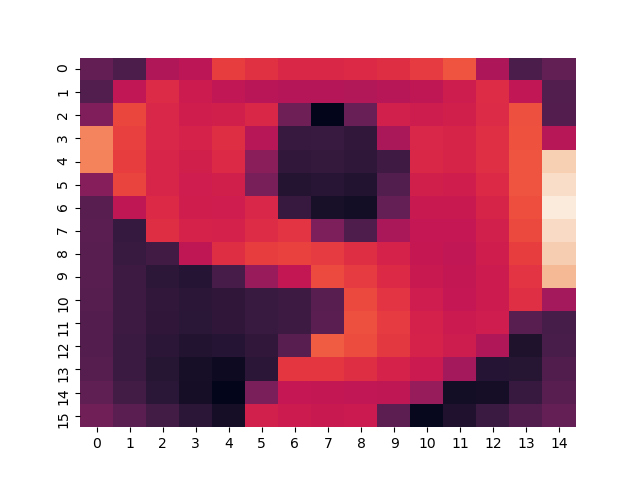
\includegraphics[scale=.15]{img/sample_original/o9}}
    \caption{Sample of the original images available in the MFDD dataset}
\label{fig:num_original}
\end{figure}

A sample of the individuals reconstructed is presented on Figure~\ref{fig:num_reconstructed}. While the MSE and the MRD are high for this view (Figure~\ref{fig:mse_b} and Figure~\ref{fig:mrd_b}), it appears visually that the reconstructed individuals can be easily recognized.

\begin{figure}[H]
    \centering
    \subfloat[][]{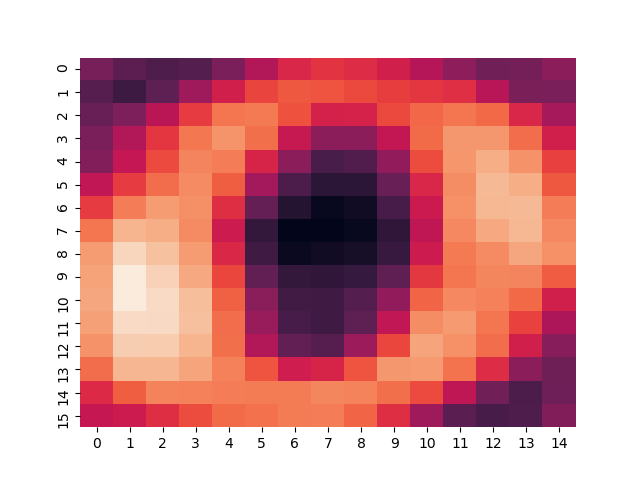
\includegraphics[scale=.15]{img/sample/0}}
    \subfloat[][]{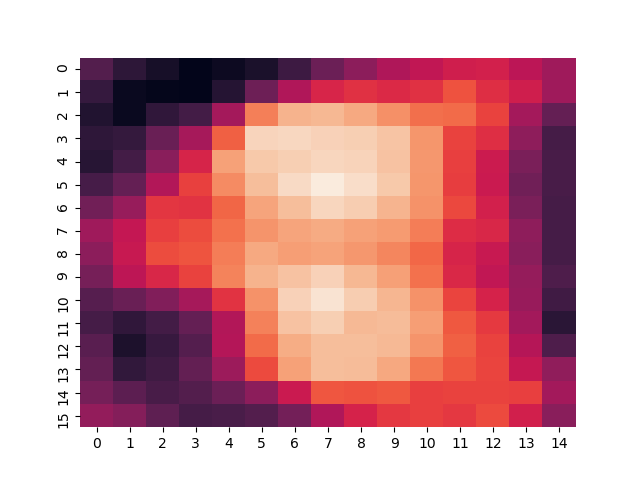
\includegraphics[scale=.15]{img/sample/1}}
    \subfloat[][]{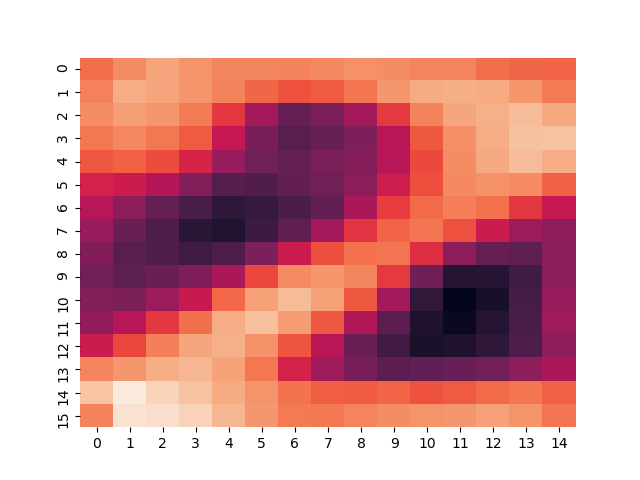
\includegraphics[scale=.15]{img/sample/2}}
    \subfloat[][]{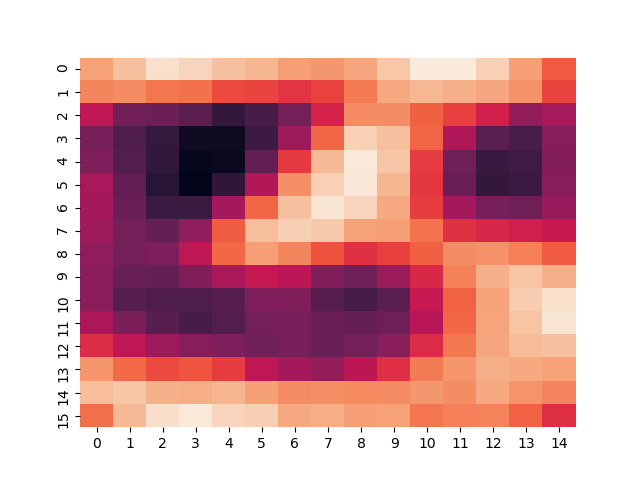
\includegraphics[scale=.15]{img/sample/3}}
    \subfloat[][]{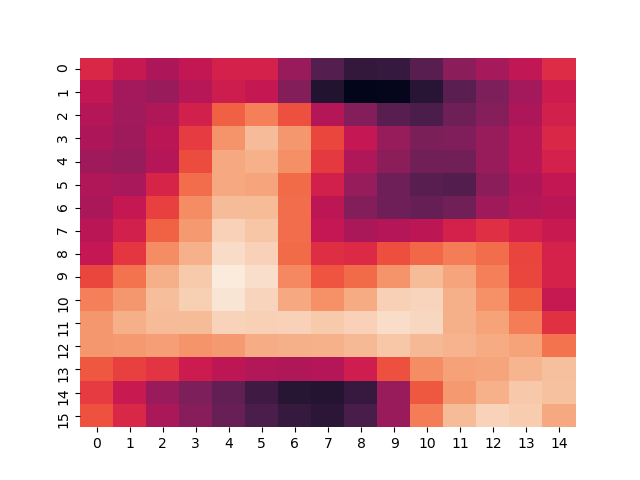
\includegraphics[scale=.15]{img/sample/4}}\\
    \subfloat[][]{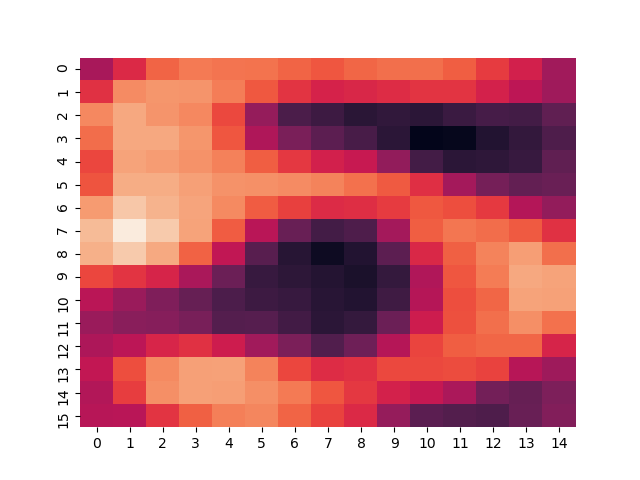
\includegraphics[scale=.15]{img/sample/5}}
    \subfloat[][]{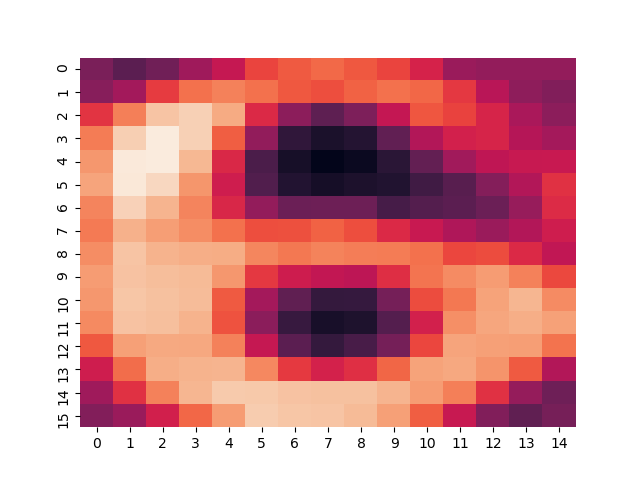
\includegraphics[scale=.15]{img/sample/6}}
    \subfloat[][]{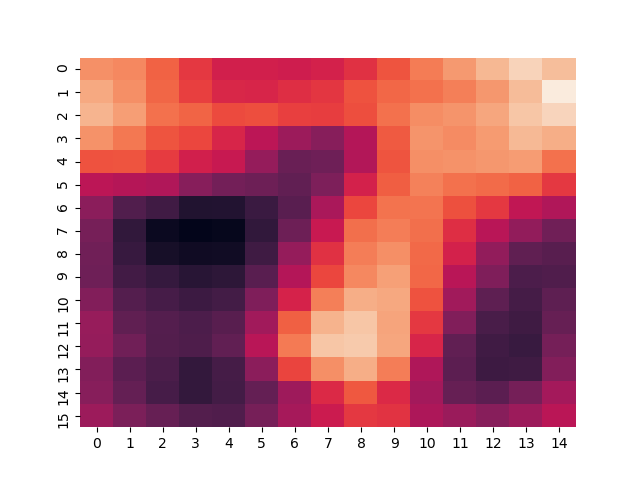
\includegraphics[scale=.15]{img/sample/7}}
    \subfloat[][]{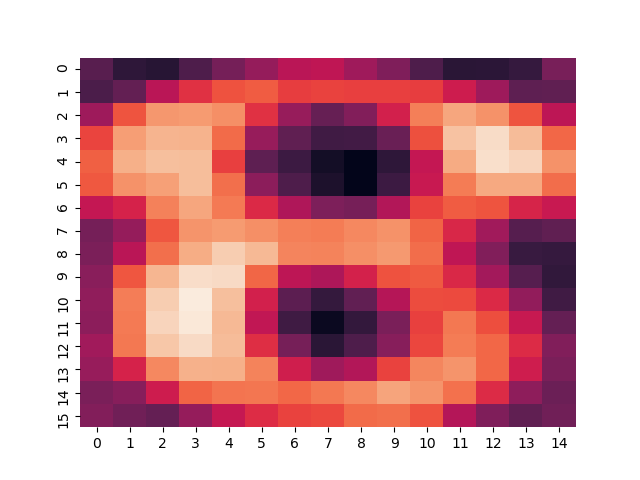
\includegraphics[scale=.15]{img/sample/8}}
    \subfloat[][]{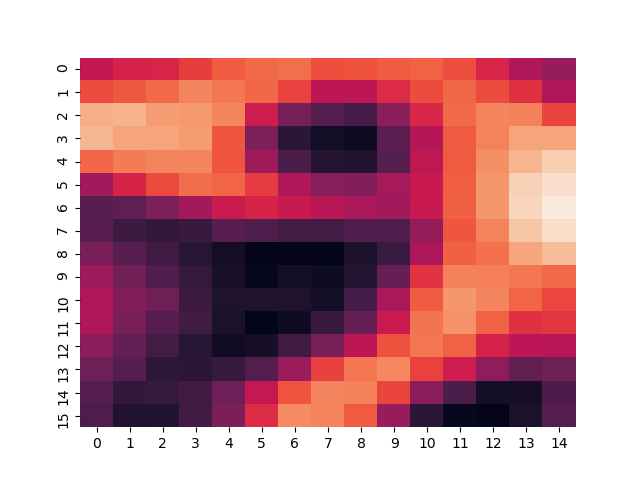
\includegraphics[scale=.15]{img/sample/9}}
    \caption{Sample of the reconstructed images available in the MFDD dataset. Some good examples.}
\label{fig:num_reconstructed}
\end{figure}

However, while it is true for most of the reconstructed images, some examples do not work as well, as presented in Figure~\ref{fig:num_reconstructed_bad}. Moreover, even if the numbers can be recognized, a blurring effect can be observed even on the best reconstructed examples. This puts forward the fact that the system approximation can be improved, because while it does not damages the recognition in the case of the MFDD dataset, we can imagine that it can damage it for some other use cases.

\begin{figure}[H]
    \centering
    \subfloat[][]{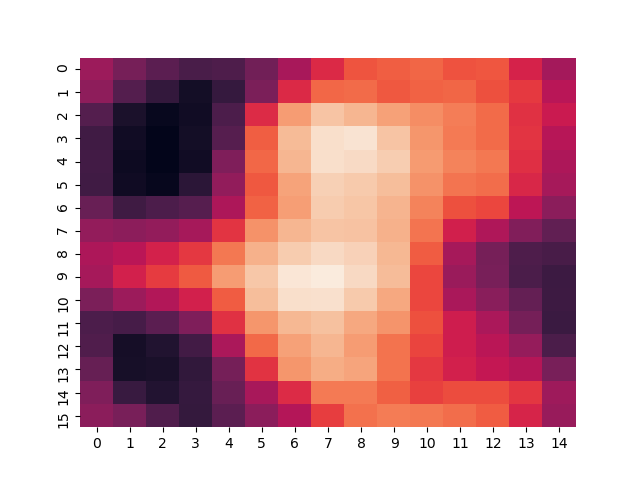
\includegraphics[scale=.15]{img/moches/00}}
    \subfloat[][]{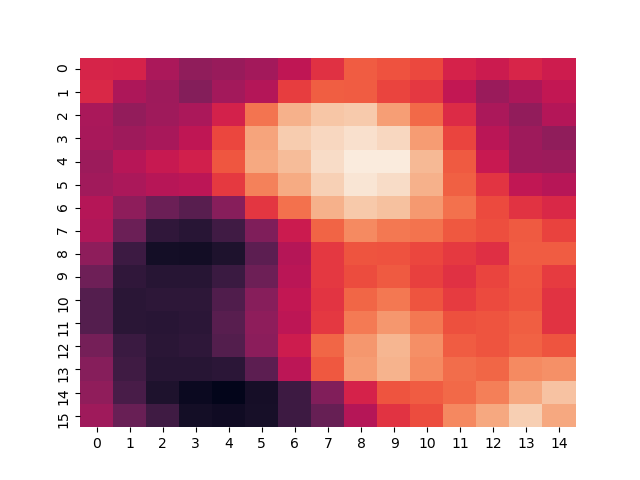
\includegraphics[scale=.15]{img/moches/11}}
    \subfloat[][]{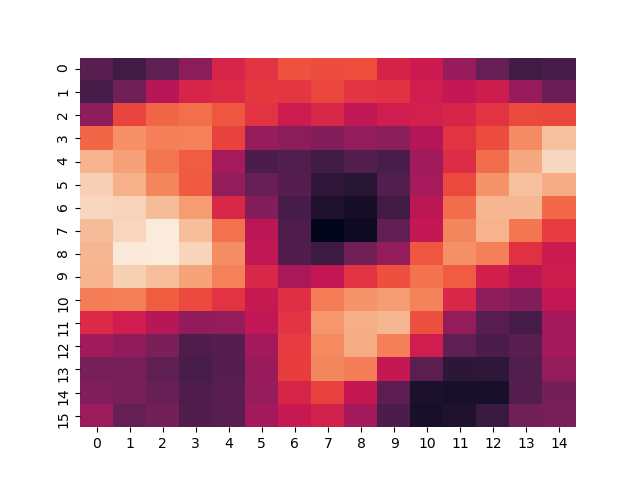
\includegraphics[scale=.15]{img/moches/22}}
    \subfloat[][]{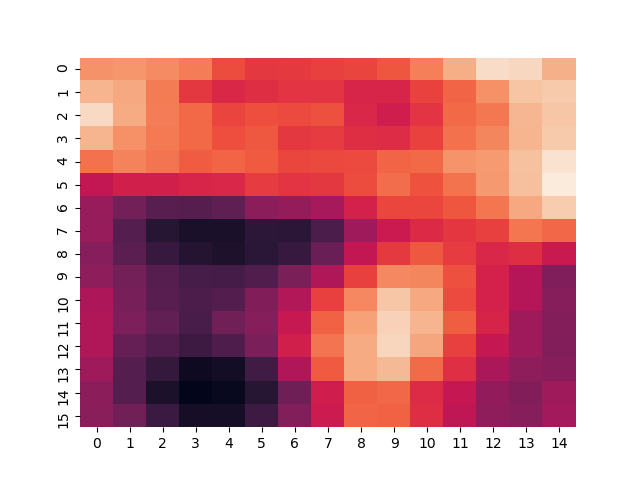
\includegraphics[scale=.15]{img/moches/33}}
    \subfloat[][]{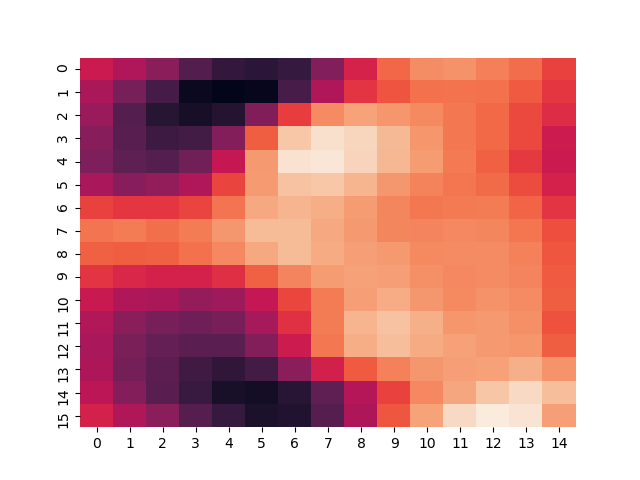
\includegraphics[scale=.15]{img/moches/44}}\\
    \subfloat[][]{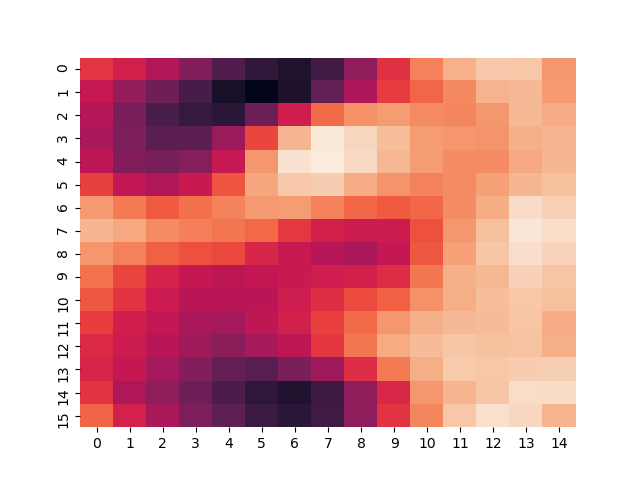
\includegraphics[scale=.15]{img/moches/55}}
    \subfloat[][]{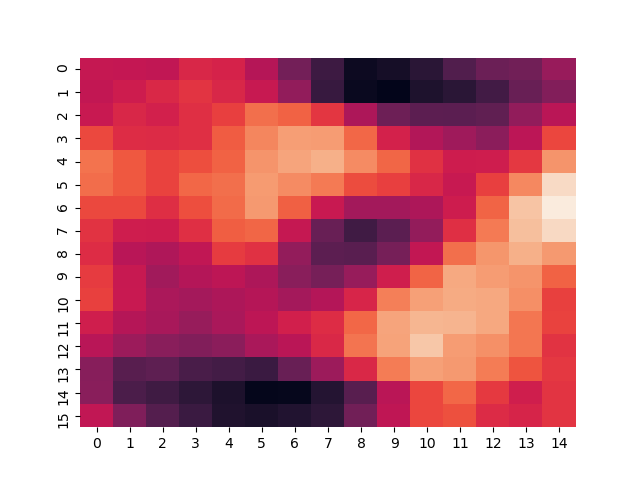
\includegraphics[scale=.15]{img/moches/66}}
    \subfloat[][]{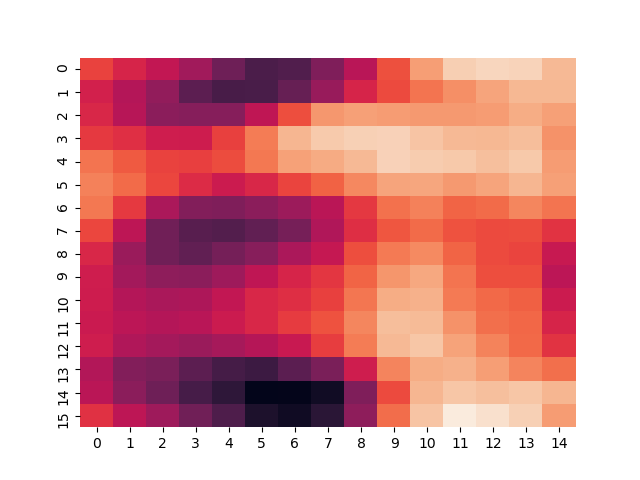
\includegraphics[scale=.15]{img/moches/77}}
    \subfloat[][]{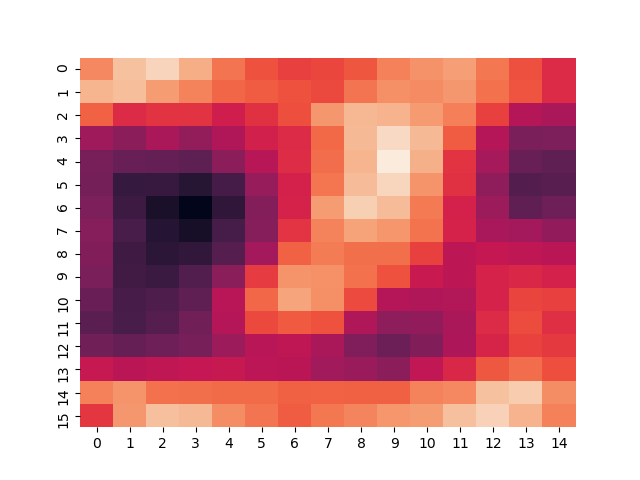
\includegraphics[scale=.15]{img/moches/88}}
    \subfloat[][]{\includegraphics[scale=.15]{img/moches/99}}
    \caption{Sample of the reconstructed images available in the MFDD dataset. Some bad examples.}
\label{fig:num_reconstructed_bad}
\end{figure}

    \subsection{Impact on the Classification Score:}
\label{sec:classif}

    For the second experiment, when looking at Table~\ref{table_classif} and Appendix~\ref{fig:classif}, we notice that the Collaborative Reconstruction System gives classification scores comparable to these obtained on the original data: for WDBC, MFDD and Cube, the maximum absolute value of the Classification Difference is 7.5\% (for the version using the Masked Weighting Method) when the mean original scores are respectively 90.9\%, 88.4\% and 75,35\%. Secondly, our new combination method damages the Classification Score for WDBC and MFDD while improving it for Madelon and Cube.\ This point has to be considered conjointly with the fact that for almost every views, our combination method tends to lower the absolute Classification Difference of each dataset.
	
\begin{table}[h]
    \centering
    \caption{Mean classification rate per database on the original data.}
\label{table_classif}
\begin{tabular}{ccccc}
\midrule
\textbf{Dataset}   & \parbox[c]{1.75cm}{\centering WDBC}  & \parbox[c]{1.75cm}{\centering MFDD}  & \parbox[c]{1.75cm}{\centering Madelon} & \parbox[c]{1.75cm}{\centering Cube}  \\ \midrule
\textbf{Mean rate} & 0.909 & 0.884 & 0.606   & 0.733 \\ \midrule
\end{tabular}
\end{table}

Even if we do not have clearly identified the source of this phenomenon, we suggest the following explanation: the quality of the output of a reconstruction system which does not use our combination method is highly dependent on the quality of the Links which make the inter-view reconstruction possible. Even if many tests have been performed for each database, the results depends on both manageable (hyperparameters of all the neural networks) and unmanageable (local minimum, initialization) points, both being very sensitive for the system training. That being said, it is very likely that the system results are very sensitive, which would explain the higher variability of the results obtained without the combination method compared to these obtained with it.\@ This latter probably tends to mitigate the variability of the results because it depends far less on sensitive points: it only requires a learning step if the gradient descent method is used to update the weights and the initialization in the same every time.

\subsection{Adaptation of the masks coefficients:}
\label{sec:results_mwm}
The point of this last set of experiments was to analyze the evolution of the masks coefficients to ensure that the method was able to determine which part of each reconstructed vector was the most useful to reconstruct the final individual. To make that possible, the Cube dataset has been generated as explained in Section~\ref{sec:datasets}, leading to the creation of 3 views each defined by 2 features. For each view, one of its feature is shared by one of the external views and the other feature is shared by the other external view. The point of this structure is to limit the mutual informations that two views can share. If the mutual information is limited to a specific set of features (the set being composed of only one feature in this example), the quality of the partial reconstructions should vary depending on the reconstructed feature, as presented in Figure~\ref{fig:process_mwm}.

In the Cube example, the information is either totally shared (same values if the feature is present in both views) or not at all (the feature not being present in the external view). Thus, we expect to obtain mask values around respectively 1 and 0. The results obtained empirically are described in Table~\ref{tab:results_mwm}. It clearly appears that the masks values adapt depending on the feature they are weighting: while these linked to the shared features are above 0.9, the ones linked to the other features never exceed 0.15. This validates the efficiency of the masks adaptation depending on the mutual information. 

\begin{table}[h]
    \centering
    \caption{Mean and standard deviation of the values of the masks coefficients depending on the feature they are weighting}
\label{tab:results_mwm}
\begin{tabular}{ccc}
\cmidrule{2-3}
\textbf{}                                       & \parbox[c]{3cm}{\centering Mean} & \parbox[c]{3cm}{\centering Standard deviation} \\ \midrule
\textbf{Shared feature}                         & 0.920    & 0.026                  \\ \midrule
\multicolumn{1}{l}{\textbf{Non shared feature}} & 0.143    & 0.034                  \\ \midrule
\end{tabular}
\end{table}

	\section{Conclusion}
\label{sec:conclusion}
In this chapter, in a global context of multiplication of multi-view data, we have presented a new system called the Cooperative Reconstruction System. The purpose of this system is to reconstruct missing data using information contained in each view, without sharing the original data, thus avoiding security issues. To do this, the system relies on three modules: Autoencoders to cipher data under a scalar vector form, Multi-Layer Perceptrons -called Links- to decipher an external code in a local view, and the Masked Weighting Method, a new weighting method to combine all external reconstructions, thus obtaining the final reconstruction. 
	
The Masked Weighting Method has three functions: combining external informations, reducing the influence of views with information which could hinder the reconstruction process, and reducing the impact of missing data during the system training process.
	
The efficiency of both our reconstruction system and our combination method has been tested on four different datasets: WDBC, MFDD, Madelon and Cube. To this end, two criterion have been considered: the adequation of the reconstructed individuals to their original versions considering using the Mean Squared Error and the Mean Relative Difference, and the impact of the use of reconstructed individuals instead of the original ones for classification purposes (tested with Random Forests).  These experiments have demonstrated the main strengths and weaknesses of the system. Its main strengths are its ability to reconstruct an individual usable in a classification task without sharing data between views as well as its ability to weight views in such a way that it improves the final result compared to a standard meaning of the external reconstructions. On the opposite, its main weaknesses are its relatively weak reconstruction scores because of the training of the Links which may be difficult depending on the original datasets, and the number of hyperparameters to set, considering that a system composed of $N$ views requires $N^2$ different neural networks to be trained.
	
To further develop the work presented in this chapter, it could be useful to study the link between the autoencoders and the MLP in charge of transfering this information. During the above experiments, the hyperparameters of each neural networks hadto be set manually. The automatic definition of such parameters, or at least the identification of a relation between a code and its use to infer information, may improve the quality of the results obtained with the Collaborative Reconstruction System.
